

\documentclass{./llncs2e/llncs}
%\documentclass[oneside]{book}


\usepackage[portuguese, english]{babel} % Português
\usepackage[utf8]{inputenc}
\setcounter{secnumdepth}{3}
\usepackage{graphicx}
\usepackage{amssymb}
\renewcommand{\labelitemi}{$\bullet$}
\usepackage[inline]{enumitem}
\usepackage{multirow}
\usepackage{chngpage}
\usepackage{pdflscape}
\usepackage{rotating}
\usepackage{eurosym}
\usepackage{longtable}
\usepackage{tabularx}

%\usepackage[titletoc]{appendix}

%\usepackage{fixltx2e}
%\usepackage{mathtools}
%\usepackage[nolist,nohyperlinks]{acronym}
%\usepackage{amsmath}%
%\usepackage{wasysym}
%\usepackage{amsfonts}%
%\usepackage{color} 
%\usepackage{colortbl}
%\usepackage{subfig}
%\usepackage{url}
%\usepackage{textcomp}
%\usepackage{rotating}
%\usepackage{threeparttable}
%\usepackage{hyperref}
%\usepackage[square,sort,comma,numbers, sort&compress]{natbib}
%\usepackage{lscape}
%\usepackage[table]{xcolor}
%\definecolor{lightgray}{gray}{0.9}
%\usepackage{tikz}
%\usepackage{gantt}
%\usepackage{mathtools}

% Maintain images and tables within their respective sections
\usepackage[section]{placeins}

% 
% Change the margins
% 
% \usepackage[margin=2.9cm]{geometry}

\begin{document}
\title{Cloud-based Facility Management Benchmarking}

\author{Sofia Martins, \\ sofia.pereira.martins@ist.utl.pt}
\institute{Instituto Superior Técnico}

\maketitle

%!TEX root = ../report.tex

% 
% Abstract 
% 

\begin{abstract}

Facilities expenditures, such as equipment maintenance or space cleaning, constitute a big slice of organizations base cost. Modern Facilities Management employs specific software such as Computer Aided Facility Management Software to identify and optimize facilities performance by benchmarking different categories of the non-core business indicators. 

A pervasive problem, however, is that organizations do not know whether they can bring those optimizations to new levels of performance, i.e. they do not know if their FM practice is in line with the performance of the best in their industry. Overall, there is a need for a benchmarking solution that could bring FM indicators of distinct facilities together, identifying the contrasts and similarities between them.

This thesis studies the problem of FM benchmarking and proposes a cloud-based solution to integrate KPI of distinct facilities. Using this solution, organizations can track their ranking in relation to other organizations, and know if they can further optimize their Facilities Management practice.


\end{abstract}
%!TEX root = ../report.tex

% 
% Keywords 
% 

\begin{keywords}

Facilities Management, Key Performance Indicator, KPI, Benchmarking, Cloud Computing, Data Analysis, Measurements, Standards

\end{keywords}
%!TEX root = ../report.tex

% 
% Introduction
% 

\section{Introduction}
\label{Introduction}

Facilities Management (FM) is a relatively new discipline, that started to be recognized in the 1970s. 
FM is a non-core activity that supports an organization to achieve its objectives (core business), making the organization more efficient, by offering employees better working conditions and rationalizing expenditures related to the facility. Thus, FM contributes to the overall performance of the organization. 

FM adoption has been growing steadily, and facilities expenditure is one of the biggest slice of the organizations base cost (maintenance costs are usually the second) \cite{Roka-Madarasz2010}.
It is important to adopt systems to measure the effect of the FM on organizations core business, together with the ones which measure the FM own performance \cite{Pitt2008}.

FM has tree main strands of activity: property management, property operations and maintenance, and office administration \cite{Pitt2008}, which are increasingly backed by specialized software such as Computer Aided Facility Management (CAFM), Building Information Models  (BIM), Computerized Maintenance Management Systems (CMMS), Computer Aided Design (CAD), Building Automation Systems (BAS), Energy Management Systems (EMS), Enterprise Resource Planning (ERP), Integrated Workspace Management System (IWMS) or some combination between them for a complementary usage. 

Through some of these software applications it is possible to extract measures and indicators, and with them calculate Key Performance Indicators (KPI). These KPIs give important insight into functioning of the FM functions (keeping track of KPIs is one aspect of quality control)  \cite{Fitz-Gibbon1990}.

Organizations have to perform better than their competitors, while operating at the lower costs. Thus, it is very important to be able to efectively compare infrastructures. With performance indicators is possible to perform a comparison between organizations. 

Benchmarking can be defined as "part of a process which aims to establish the scope for, and benefits of, potential improvements in an organisation through systematic comparison of its performance with that of one or more other organizations" \cite{EN15221-7}. Benchmarking can be used either for comparison between distinct organizations or for comparison between facilities within the same organization, also a facility can be compared with itself at different time lines.

Benchmarking brings many advantages:
 \begin{enumerate*}[label=\itshape\roman{enumi})]
  	\item justification of energy consumption, costs and practices,
  	\item identification of weaknesses/ threats, strengths/ opportunities and best practices,
  	\item addition of value to facilities integrating them in CAFM systems and supporting maintenance management. 
\end{enumerate*}
Therefore, benchmarking can be seen as an instrument to measure facilities performance, and performance indicators are very important for the FM benchmarking. 
% The main facility-oriented benchmarking indicators are related to flexibility, space usage, maintenance management, safe environment and value for money \cite{Gilleard2004}.
%Therefore, they are very important for the FM benchmarking.

Up to now, the comparison between organization is not yet possible. Although some organizations have their own benchmarking software, this software is not compatible between distinct organizations. There is no centralized mechanism to integrate all these data. Results from them are not in the same format or have not the same KPIs. Furthermore, is still not clear which are the most important KPIs that should be used by each sector organizations. The same holds for the field of FM.

Another recent trend is cloud solutions that are being employed successfully for benchmarking in sector such as financial, maintenance and space. There are several technologies that can be used such as Infrastructure as a Service (IaaS) where the consumer has the capability to acquire processing, storage, networks, and other fundamental computing resources, Platform as a Service (PaaS) where the consumer has the capability to deploy his solution onto the cloud infrastructure or Software as a Service (SaaS) where applications are accessible from various client devices \cite{Lenk2009}. 
These cloud solutions present several benefits such as saving of IT costs and maintenance (since it is not necessary any installation of equipment or software, and neither their maintenance by the organization IT sector), strong integration capabilities, short time-to-benefit, and scalable computation on demand that keep up with the customer needs. Specifically in benchmarking, cloud applications permits a easier way for entering and process the data, and can be accessible by everyone and anywhere. 

A benchmarking application that enables organizations to send facilities related information in standardized format to be processed and presented graphically is a valuable addition, since it enables that every organization benchmark results can be compared with each other (by creating interfaces that can communicate with the software that captures the measurements). This makes possible a raking between them, which would generate a healthy competition that motivates the improvement of each organization FM.

Therefore, the central motivation for this work is to study the migration of facilities benchmarking to the cloud using the latest computing technologies and design a solution, where a cloud application would receive all important data from multiple sources, this data will correspond of various metrics necessary for the calculation of a set of KPIs that will be identified through an analysis of related work. Through the previous information, the solution would also carry out a benchmark comparison between distinct organizations in the industry according to the obtained Key Performance Indicators (KPIs).

\subsection{Motivation}

Consider a cloud solution that aggregates benchmarking information of distinct facilities, and ranks them according to their performance. Facilities managers would have a deeper insight of their own FM areas. 
%Facilities would be more and more optimized, in a way that they would compete healthily between them for a better FM in their organizations.

\begin{quote}
	{\bf Scenario 1} Consider an organization that has applied FM and where benchmarking has been applied for some time now. This organization decides to use the application proposed in this document. Through it, verifies that its position is raking well below than expected. Thus, seeing their ranking, they become motivated to improve (as they have a perception of their space for improvement) both globally and at the level of a particular indicator.
\end{quote}

\begin{quote}
	{\bf Scenario 2} Consider two distinct organizations that are using the cloud application presented in this document. The first organization has been on the raking first place for some time now. However, the second organization took their place in the raking, but the first organization wants to regain its position. Thus, it creates a healthy competition among participants (who do not know the identity of the other), where improvement is still driven dynamically.
\end{quote}

There are some solutions to address this goal, however, none of them are so simple to use. Today's solutions are difficult to use, information is difficult to read and understand, and none of them can give you your position in the market relatively your organizations competition.

\subsection{Problem Statement}
As we made clear before, there is not an agreement about which KPI should be applicable in each sector. According to Hinks and McNay \cite{Hinks1999}, the lack of generalized sets of data and industry wide sets of KPIs results on poor comparability of performance metrics across organizations and industries. Furthermore, there still is a lack of solutions for FM that enable integrating data from different organization in a way that brings gains for them. 
Organizations continue to use distinct software to their FM and KPI gathering, which difficult the aggregation and analysis of all data. 

Our hypothesis is that a cloud-based and vendor-independent FM solution for benchmarking will enable organizations to know their positioning and also to compare the performance of distinct facilities (in the case of facilities managed by the same entity), through a set of metrics provided by the facilities managers. To this end, it is also necessary to know what is the list of KPIs that should be used to benchmarking distinct facilities.


\subsection{Methodology and Contributions}

The methodology of this document will include the analysis of standard benchmarking surveys and the systematization of most commonly used indicators in FM. These indicators will undergo a prioritization to identify the most relevant. The prioritization will make use of scientific studies, existing standards for FM, and the help of FM experts, analyzing the most important indicators on a theoretical and practical level. Finally, the architecture of a cloud-based solution for FM benchmarking will be presented, that enables organizations to compare their results with others. More specifically, the contributions of this document are:
\begin{itemize}
	%\item explanation of the main subjects and concepts
	\item A comparative study between the different Facilities Management standards
	\item The evaluation and comparison between the main FM benchmarks and the indicators produced
	\item The identification of the main benchmarking indicators of interest
	\item A survey of the main FM tools
	\item The design of the architecture of the cloud benchmarking application and its implementation.
	%\item respective cloud application evaluation.
\end{itemize}


%!TEX root = ../report.tex

% 
% Objectives
% 

\section{Concepts}
\label{Concepts}

This section discusses key aspects of Facilities Management, Benchmarking and Cloud applications.

\subsection{Facilities Management}
\label{FacilitiesManagement}

Core activities are bound to the central business of the organization and its strategy. While the non-core activities are not necessarily required by an organization in fulfilling its value proposition to its customers, and can be outsourced to third parties (such as security, payroll, cleaning, maintenance of the building, catering, printing, vehicle maintenance or conference facilities). 

Facility Management (FM) is a non-core activity that supports an organization in the pursuit of its objectives (core business), and is considered ``the practice of coordinating the physical of business administration, architecture, behaviour and engeneering science" \cite{IFMA} by the International Facility Management Association (IFMA). FM is a result-oriented management of facilities and services securing best value in the provision of services, making the organization more efficient, by giving better conditions and making less expenditures.

FM is supported by specialized software such as Computer Aided Facility Management (CAFM) packages that track space usage, cable pathways, employee locations, security and access control.

CAFM systems are often integrated with Computer Aided Design (CAD), important to support the planning and monitoring of spaces and activities in it, and a database back-end that contains non graphical data about the spaces. CAFM software also enables managing changes to the space since can be tried and tested in computer before they are made, which can avoid future problems. 
CAFM systems can be populated from Building Information Models (BIM) information containing geometry, spatial relationships, geographic information, quantities and component properties \cite{Atkin2009}, also interfaces to other systems such as a Computerized Maintenance Management Systems (CMMS) to manage preventive maintenance activities. They also have the ability to help decrease the time for task request to task completion, increase the speed and accuracy of information related to each task, and provide improved cost and trend analysis \cite{May2012}. 

These systems bring along several benefits as: 
\begin{enumerate*}[label=\itshape\roman{enumi})]
	\item efficient completion of operational sequences (entry and analysis of data),
	\item increase the productivity of workers (by determining property improvements),
	\item potential cost savings (in areas such as cleaning contracts and energy consumption),
	\item analysis of information on costs,
	\item supporting management decisions, 
	\item precise valuation of fixed assets,
	\item optimization of space utilization.
\end{enumerate*}

Beyond this type of software, there are others like Incident Management Systems (IMS) that are used by operators (which register incidents) or technicians (who deal with occurrences and close them) to register, centralize and follow each occurrence's status. These systems can generate an automatic work backlog for each technician, which provides work efficiency. It also has reporting services, statistics, incidents status, etc. IMS can be integrated with CMMS or with incident management systems from third party service suppliers to fill-in work order requests.

Computerized Maintenance Management Systems (CMMS) creates and associates maintenance plans, that can be grouped by type of device, for each equipment of an organization, such as air conditioning, roller stairs, furnitures, etc. Some CMMS assist in performing contract management and equipment management. Some of CMMS can be integrated with BAS to obtain equipment usage metrics, however some information can not be possible to retrieve directly from BAS, but it is possible using gathering devices.

Building Automation Systems manage every building's environment aspect, automatically controlling devices installed in the building. Facility managers can remotely command and supervise automation sub-systems in real-time. BAS keeps a history log of the status of each device and defines alarm conditions that can be used to detect malfunction symptoms or devices failure, and can be integrated to CMMS or CAFM tools to report space usage metrics obtained from occupancy sensors.

Energy Management Systems (EMS) gathers all energy consumption information from energy meter devices installed along the building such as electric current consumption. This information can be analyzed in detail and enables facility managers to analyze consumption variation within comparable periods of time. BAS and EMS can be connected together to create consumption profiles and determine relative contribution of devices or groups of devices to the overall energy consumption.

However Enterprise Resource Planning (ERP) systems are not considered FM applications, they are very important on FM environment where management of suppliers, logistics, accounting, billing and orders is being made. 

Integrated Workspace Management System (IWMS) suites integrate functionalities of an ERP for FM with CAFM and CMMS in one single application. The organization of all these softwares referred above can be seen on Figure \ref{fig:ClassesFMApps}.

\begin{figure}[t!]
  \centering
  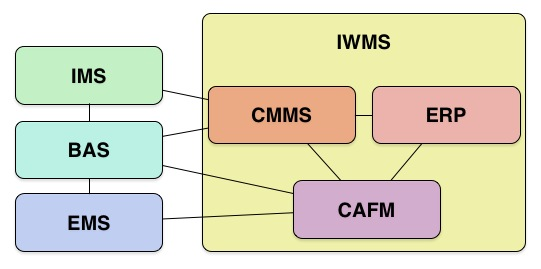
\includegraphics[width=0.95\textwidth]{img/ClassesFMApps.jpg}
  \caption{Organization of the six classes of software applications for FM. The interoperability between the classes is represented by a line between them. IWMS is a group composed by the three classes: CMMS, ERP and CAFM.}
  \label{fig:ClassesFMApps}
\end{figure}

Most of these systems today are web-based enabling an easier entering of the facilities data that can be analyzed and consulted anywhere. These analysis and benchmarking of all data results in Key Performance Indicators (KPIs) over a core of skills that are aligned with business objectives as a way to measure current levels of performance and achievement. 

\subsection{Benchmarking}

Benchmarking has been defined has the search of ``industry best practices that lead to superior performance" by Camp \cite{Camp1989}. It is an important process to compare performance aspects such as operating costs, maintenance and cleaning activities, space utilization, energy consumption or administrative costs. It uses different previously established metrics, identifies differences, alternative approaches and assess opportunities for improvements and change. Overall, it is a process that gives organizations instruments to know how they are performing both internally and to costumers.
 
Benchmarking can bring many advantages for a facility such as:
\begin{enumerate*}[label=\itshape\roman{enumi})]
	\item not waste time and costs when someone else has already done it better, faster and cheaper,
	\item increase the velocity of change and restructuring,
	\item improvement in and off itself, by forcing organizations to examine present processes,
	\item more likely implementation, because process owners are more involved.
\end{enumerate*}

Historically FM started with a focus on performance measurement, that had three broad purposes: 
\begin{enumerate*}[label=\itshape\roman{enumi})]
	\item ensure the achievement of goals and objectives, 
	\item evaluate, control and improve procedures and processes, 
	\item compare and assess the performance of different organizations, teams and individuals. 
\end{enumerate*}

Over the years, however, attentions shifted to quality and consumer satisfaction \cite{Pitt2008}, for this end, benchmark has a set of goals such as better prioritize and allocate resources, and identify opportunities, but it has a major goal: performance improvement of the organization. To this end, there is a set of requirements such as:
 \begin{enumerate*}[label=\itshape\roman{enumi})]
	\item know what clients require for the organization process,
	\item key stakeholders have to be involved in the benchmarking process,
	\item there can not be change resistance,
	\item results are not instantaneously.
\end{enumerate*}

% The focus of FM skills and techniques should be in the area that contributes to the overall management of a business by relating accommodation and support infrastructure issues to business, financial and personal criteria \cite{Pitt2008}. There is a need to assess performance in order to guide management decision-making (performance measurement is a driver to an innovation process in an organization). 

Benchmarking is not as simples as the aggregation of a few indicators. There must be meaning for each one of them, a purpose for choosing each one. Camp lists four fundamental steps for benchmarking \cite{Camp1989}:
\begin{itemize}
	\item {\bf Knowing operation} to evaluate internal operation strengths and weaknesses.
	\item {\bf Knowing the industry leaders or competitors} to know the strengths and weaknesses of the competition.
	\item {\bf Incorporating the best} to emulate the strengths of the leaders in competition.
	\item {\bf Gaining superiority} to go beyond the best practices installed and be the best of the best.
\end{itemize}

Clearly, the FM benchmarking process requires a planning phase that decides which data to collect \cite{Gilleard2004}.

\subsection{Key Performance Indicators}

Performance Indicators are collected in many complex systems which, such as education, deliver a service \cite{Fitz-Gibbon1990}. These indicators are not perfect measures, without error or problems of definition and interpretation, but they are important pointers to the functioning of the system and keeping track of them is one aspect of quality control \cite{Fitz-Gibbon1990}.

The first step of benchmarking is the establishment of performance objectives and metrics. For example, the number of tasks completed in a given time interval. Just like all the actions that must be well performed to accomplish satisfactorily those objectives or goals. All these are important for all measurements and performance comparison between benchmarking parties, but it is important to know that the choosing of wrong indicators can be damaging, and therefore, it is also important to know that Measurements and Indicators are distinct concepts. Measurements are a direct representation of the scale of the organization and are direct measurable items (for organizations internal usage) while Indicators are quantifiable metrics that reflects organizations goals achievement (external usage). It is important to distinguish Performance Indicators (PI) from Key Performance Indicators (KPI). The PIs tells you what to do, while the KPIs tells you what to do to increase performance dramatically, so, they represent a set of measures focusing on most critical aspects of organizational performance for the current and future success of the organization \cite{Parmenter2007}.

KPIs are not the same for all the sectors and employees on an organization. Associated directors or head of advisors have custom KPI for their specific responsibilities. Also, there are various generic KPIs for other professionals and managerial personel based on business measures. However, they all must be SMART \cite{Arash2007}:
\begin{itemize} %Specific, Measurable, Attainable, Realistic, Time-sensitive
	\item {\bf Specific} well defined and clearly understood.
	\item {\bf Measurable} theres a well defined process that enables the KPI tracking.
	\item {\bf Attainable} must be able to be met with the resources available.
	\item {\bf Realistic} that can be measured at a reasonable cost.
	\item {\bf Time driven} if corresponds of a time interval.
\end{itemize}

Therefore, FM departments must have their own KPIs that are aligned with the core business KPIs \cite{Teicholz2001}. The main typical FM KPIs (over a unit of time) according to Teicholz \cite{Teicholz2001} are: 
\begin{enumerate*}[label=\itshape\roman{enumi})]
	\item Operational Hours,
	%\item Areas of Responsibility,
	\item Response Times,
	\item Rework,
	\item Value Added,
	\item Number and performance of suppliers,
	\item Employee satisfaction,
	\item Innovations (new processes),
	\item Customer satisfaction,
	\item Plan versus actual on contracts,
	\item Number of items on tasks lists
\end{enumerate*}.

\subsection{Cloud Computing}

Cloud Computing is arising and being applied to various fields. It provides environments to enable resource sharing in terms of scalable infrastructures, middleware and application development platforms, and value-added business applications \cite{Zhang2009}.



%\subsubsection{Cloud Computing Concepts}
%\hfill \\ 
The Cloud is an aggregation of a set of resources such as networks, servers, applications, data storages and services, in only one place, which the end user can access and use with minimal management effort or service provider interaction. 
The main goal of Cloud Computing is to make a better use of distributed resources, combine them to achieve higher throughput and be able to solve large scale computation problems.
%The cloud architecture can be private (hosted within an organization's firewall) or public (hosted on external cloud providers).

% for which contributes the following characteristics:

% \begin{description}
% 	\item [On-demand self-service] permits that a consumer can acquire computing capabilities, such as server time and network storage, as needed automatically without requiring human interaction with each service provider.\\

% 	\item [Broad network access] in the sense that capabilities are available over the network and accessed through standard mechanisms that promotes heterogeneous use by thin and thick client platforms (e.g., mobile phones, tablets, laptops, and workstations).\\

% 	\item [Rapid elasticity] means that computing capabilities can be elastically provisioned and released, in some cases automatically, to scale rapidly outward and inward commensurate with demand. To the consumer, the capabilities available for provisioning often appear to be unlimited and can be appropriated in any quantity at any time.\\

% 	\item [Computing resources pool] to serve multiple consumers using a multi-tenant model, with different physical and virtual resources dynamically assigned and reassigned according to consumer demand. There is a sense of location independence in that the customer generally has no control or knowledge over the exact location of the provided resources but may be able to specify location at a higher level of abstraction (e.g., country, state or data-center). Examples of resources include storage, processing, memory, and network bandwidth.\\

% 	\item [Measurement services] to control and optimize resource use by leveraging a metering capability at some level of abstraction appropriate to the type of service (e.g., storage, processing, bandwidth, and active user accounts). Resource usage can be monitored, controlled, and reported, providing transparency for both the provider and consumer of the utilized service.


% \end{description}


\subsubsection{Cloud Computing Concepts} 
\hfill \\ \\
Today we have several services that we can use, since Infrastructure as a Service (IaaS), Platform as a Service (PaaS) or Software as a Service (SaaS) \cite{Lenk2009}.

\begin{description}
	\item [Infrastructure as a Service (IaaS)] the consumer has the capability to acquire processing, storage, networks, and other fundamental computing resources where the consumer is able to deploy and run arbitrary software, which can include operating systems and applications. An example is Amazon EC2 which provides web service interface to easily request and configure capacity online \cite{ec2}. For a higher layer of IaaS, computational, storage, and network an example is Amazon’s Dynamo \cite{DeCandia2007}.\\

	\item [Platform as a Service (PaaS)] the consumer has the capability to deploy onto the cloud infrastructure, consumer-created or acquired applications created using programming languages, libraries, services, and tools supported by the provider. An example is Google’s App Engine \cite{GoogleAppEngine} and Heroku \cite{Heroku}.\\

	\item [Software as a Service (SaaS)] the applications are accessible from various client devices through either a thin client interface, such as a browser, or a program interface. The consumer does not manage or control the underlying cloud infrastructure including network, servers, operating systems, etc.

\end{description}
% IaaS have two distinguish services: Physical Resource Set (PRS) and Virtual Resource Set (VRS), which both provide a management front-end API, however, PRS layer is hardware dependent. So, splitting these two resources allows automated management of physical as well as virtual resources. Examples of PRS resources are Emulab \cite{Hibler2008} and iLO \cite{ILO}, while examples of VRS are Amazon EC2 which provides web service interface to easily request and configure capacity online \cite{ec2}, Eucalyptus \cite{Nurmi2009} or OpenNebula \cite{Sotomayor2008}.

% At a higher layer of IaaS we have Basic Infrastructure Services (BIS), computational, storage, and network, like system as MapReduce \cite{Dean2008}, GoogleFS \cite{Ghemawat2003} or OpenFlow \cite{Mckeown2008}. Even higher on IaaS layers we have Higher Infrastructure Services (HIS) like Amazon’s Dynamo \cite{DeCandia2007} and Google’s Bigtable \cite{Chang2008} that are built on top of BIS.

% PaaS can be seen divided into Programming Environments like Django Framework \cite{Django} and Execution Environments like  Google’s App Engine \cite{GoogleAppEngine}.

% SaaS, for other hand, can be seen like all the cloud applications that provide a direct service to the client, and can be split into Basic Application Services like OpenId \cite{openId} and Composite Application Services like Google Maps \cite{GoogleMaps}.

The application developers can either use the PaaS layer to develop and run their applications or directly use the IaaS infrastructure \cite{Lenk2009}.

% \subsubsection{Cloud Computing Deployment Methods}
% \hfill \\ All Cloud services, from computing power to computing infrastructure, applications, business processes to personal collaboration, can be developed and deployed in several different ways:

% \begin{description}
% 	\item [Private cloud] system infrastructure is provisioned for exclusive use by a single organization comprising multiple consumers (e.g., business units). It may be owned, managed, and operated by the organization, a third party, or some combination of them.\\

% 	\item [Community cloud] system infrastructure is provisioned for exclusive use by a specific community of consumers from organizations that have shared concerns (e.g., mission, security requirements, policy, and compliance considerations). It may be owned, managed, and operated by one or more of the organizations in the community, a third party, or some combination of them, and it may exist on or off premises.\\

% 	\item [Public cloud] system infrastructure is provisioned for open use by the general public. It may be owned, managed, and operated by a business, academic, or government organization, or some combination of them. It exists on the premises of the cloud provider. Examples of public cloud providers are: Salesforce.com, Amazon Web Services and Luna Cloud.\\

% 	\item [Hybrid cloud] system infrastructure is a composition of two or more distinct cloud infrastructures (private, community, or public) that remain unique entities, but are bound together by standardized or proprietary technology that enables data and application portability (e.g., cloud bursting for load balancing between clouds).

% \end{description}

%\subsubsection{Cloud Computing Benefits}
% \hfill \\ 
In short, cloud solutions present several benefits that keep up with the customer needs such as saving of IT costs and maintenance, easy access and up-to-date data, short time-to-benefit, improving business processes and scalable computation on demand. 
These benefits have pushed many residential and commercial solutions to the cloud. 

%Hence, based on our research across publications, research projects, and industry trends (e.g., IMC-AESOP, IMS2020, Industry 4.0, Internet of Things, Cyber-physical systems), we believe that the industrial sector will also incorporate cloud technologies in their energy management and production processes.

% \begin{description}
%  	\item [Saving of IT costs and maintenance] because it allows to avoid overhead costs on acquiring and maintaining hardware, software, and IT staff.\\

%  	\item [Easy access and up-to-date data] because applications can be easily accessed from anywhere in the world with an Internet connection and a browser, i.e., without having to download or install anything.\\

%  	\item [Short time-to-benefit] with quick deployment of IT infrastructures and applications. The software deployment times and resource needs associated with rolling out end-user cloud solutions are significantly lower than with on-premise solutions.\\

%  	\item [Improving business processes] with better and faster integration of information between different entities and processes.\\

%  	\item [Scalable computation on demand] to overcame constant environments and usage changes.

% \end{description}

% Also, cloud computing is efficient for medium enterprises


%\subsubsection{Cloud Computing Risks and Concerns}
%\hfill \\ 
As all new technology arrives, it brings with it some issues which may prove to be disastrous if not taken care of. The major concerns about cloud computing are security and privacy, network performance and reliability.

% \begin{description}
% 	\item [Security and privacy] Having to share an infrastructure with unknown outside parties, requires a high level of assurance in the security mechanisms used for logical separation. 
% 	%One way to handle this concern is by using a proper cloud deployment architecture, such as hybrid clouds (with sensitive data kept on-premise) or with a private cloud and with the use of proper authentication techniques such as secure and encrypted connections (TLS/SSL with X.509 digital certificates), encrypted data storage techniques (using AES-256 military encryption), authentication and identity management (using Active Directory/LDAP services), end-to-end data integrity (using SHA-1, Secure Hash Algorithm), and private retained keys (ensures that all information requests must involve the owner). \\

% 	\item [Network performance] Real-time monitoring systems are hard to implement in the cloud due to latency issues. The term latency refers to the time that takes between the interaction and final response. 
% 	%In a local network, data is constantly flowing back and forth through servers, routers, switches and other hardware. Moving or accessing data to or from a cloud data center, will involve passing through the cloud provider network (which it is up to the cloud provider to decide their speed and quality of service) that can be overloaded and through extra security layers, i.e. firewalls. The increased and unpredictable latency can lead to a very unsatisfactory real-time experience, cause errors, or affect the productivity of production lines. \\

% 	\item [Reliability] Servers can crash, connections can go down, and the more connections there are the more possibilities there are for disconnections. The more dependent customer critical production processes are from the cloud, the more dependent the customer is from the cloud Quality of Service (QoS). 
% 	%If something goes wrong with the cloud system, the customer must wait for the cloud provider IT staff to fix it, and in meanwhile production processes can stop and cause lost in revenues.
% \end{description}


However, if the correct service model (IaaS, PaaS, or SaaS) and the right provider is selected, the payback can far outweigh the risks and challenges. The cloud implementation speed and ability to scale up or down quickly, means companies can react much faster to changing requirements like never before.

\subsubsection{Cloud Computing for FM}
\hfill \\ \\ With Cloud Computing it is not necessary installation of any software on the organization IT equipment, thus, there are no infrastructure requirements and because the service is sold on-demand, it can be rented rather than bought. Also, cloud applications are managed and updated by the provider, who take care of server maintenance and security issues. This removes burden of the IT group, and consequently, lower costs.

Because cloud enables the access of applications with both mobile or desktop devices, personnel can work flexibly anywhere and anytime. Work traveling restrictions such as different time zones or impossible access to the software are no longer an issue.

%Concluding, cloud computing brings a set of new features that increase the workforce and operational efficiencies, also improves the cash flow.

%The bottom line is that cloud-based facilities and space management apps increase workforce and operational efficiencies, and improve cash flow. In a recent study, Gartner projected that by 2016 36% of all data will be stored in the cloud. Make 2014 the year for your company to reap the benefits of cloud-based facilities and space management. To find out more about how this approach could work for you, click the link below:







%!TEX root = ../report.tex

% 
% Related work
% 

\section{Related Work}
\label{RelatedWork}

This section discusses standard organizations and benchmarking standards for FM. Also, an overview of existing benchmarking solutions such as ARCHIBUS and PNM Soft Sequence Kinetics is described. The scientific literature is also presented in this section along with a discussion of the normalization and prioritization of KPIs. 


\subsection{ISO and ICS}
The International Organization for Standardization (ISO) is the largest developer of voluntary International Standards covering all aspects of technology and business. ISO has formed joint committees to develop different kinds of standard according to the commission they join: IEC-International Electrotechnical Commission or ASTM-American Society for Testing and Materials. 
The International Classification for Standards (ICS) is a structure for catalogs of international, regional and national technical standards and other normative documents developed and maintained by ISO. It covers every economic sector and activity where these technical standards can be used. Its objective is to facilitate the harmonization of information and ordering tools \cite{ICS2005}.

Thus, we selected the most important standards for FM and Maintenance for those working with facilities in various stages of their life cycle, which are shown in Table \ref{tb:TableISO}, ordered by ICS.
\begin{landscape}
\begin{table}[h!]

		\centering
		\vspace{-2cm}
		\begin{adjustwidth}{0,5cm}{0cm}% adjust the L and R margins by 1 inch
		\resizebox{18cm}{!} {
			\begin{tabular}{ll}
				\hline
				{\bf Code} & {\bf Title} \\ 
				\hline

				{\bf ICS 01. 110: Facilities Management} &  \\
				ISO/CD 18480-1  & Part 1: Terms and definitions \\
				ISO/CD 18480-2  & Part 2: Guidance on strategic sourcing and the development of agreements \\
				\hline

				{\bf ICS 01. 110: Document Management} &  \\
				EC 82045-1:2001  & Part 1: Principles and methods \\
				IEC 82045-2:2004  & Part 2: Metadata elements and information reference model \\
				ISO 82045-5:2005 & Part 5: Application of metadata for the construction and facility management sector \\ 
				\hline

				{\bf ICS 03. 100: Risk Management} & \\
				ISO 31000:2009 & Principles and guidelines \\           
				ISO/TR 31004:2013  & Guidance for the implementation of ISO 31000 \\  		  
				IEC 31010:2009  & Risk assessment techniques \\  
				\hline

				{\bf ICS 03. 100: Asset Management}  & \\
				ISO 55000:2014 & Overview, principles and terminology \\ 	            
				ISO 55001:2014 & Management systems-Requirements \\		            
				ISO 55002:2014  & Management systems-Guidelines for the application of ISO 55001 \\  
				\hline

				{\bf ICS 03. 080: Outsourcing} & \\
				ISO/DIS 37500 & Guidance on outsourcing \\ 
				\hline

				{\bf ICS 91. 010: Building Information Modeling} & \\
				ISO/TS 12911:2012 & Framework for building information modeling (BIM) guidance \\ 		        
				ISO 29481-1:2010 & Information delivery manual-Part 1: Methodology and format \\	            
				ISO/AWI 29481-1 & Information delivery manual-Part 1: Methodology and format \\	            
				ISO 29481-2:2012 & Information delivery manual-Part 2: Interaction framework \\
				\hline

				{\bf ICS 91. 040: Buildings and Building Related Facilities}  & \\  
				ISO 11863:2011 & Functional and user requirements and performance -- Tools for assessment and comparison \\
				\hline

				{\bf ICS 91. 040: Buildings and Constructed Assets}  & \\
				ISO 15686-1:2011 & Service life planning-Part 1: General principles and framework \\
				ISO 15686-2:2012 & Service life planning-Part 2: Service life prediction procedures \\		            
				ISO 15686-3:2002 & Service life planning-Part 3: Performance audits and reviews  \\		            
				%ISO/CD 15686-5 & Service life planning-Part 5: Life-cycle costing  \\         
				ISO 15686-5:2008 & Service life planning-Part 5: Life-cycle costing  \\	            
				%ISO/AWI 15686--7 & Service life planning-Part 7: Performance evaluation for feedback of service life data from practice  \\		            
				ISO 15686-7:2006 & Service life planning-Part 7: Performance evaluation for feedback of service life data from practice  \\	            
				ISO 15686-8:2008 & Service life planning-Part 8: Reference service life and service--life estimation \\		            
				ISO/TS 15686-9:2008 & Service life planning-Part 9: Guidance on assessment of service--life data  \\		            
				ISO 15686-10:2010 & Service life planning-Part 10: When to assess functional performance \\		            
				ISO/DTR 15686-11 & Service life planning-Part 11: Terminology \\
				\hline

				{\bf ICS 91. 040: Buildings Construction}  &  \\
				ISO 15686-4:2014 & Service Life Planning -- Part 4: Service Life Planning using Building Information Modeling \\		            
				ISO 6242-1:1992 & Expression of users' requirements-Part 1: Thermal requirements  \\		            
				ISO 6242-2:1992 & Expression of users' requirements-Part 2: Air purity requirements  \\		            
				ISO 6242-3:1992 & Expression of users' requirements-Part 3: Acoustical requirements \\
				\hline

				{\bf ICS 91. 040: Performance Standards in Building}  & \\
				ISO 6240:1980 & Contents and presentation  \\	            
				ISO 6241:1984 & Principles for their preparation and factors to be considered  \\		            
				ISO 7162:1992 & Contents and format of standards for evaluation of performance  \\		            
				ISO 9699:1994 & Checklist for briefing-Contents of brief for building design  \\			            
				ISO 9836:2011 & Definition and calculation of area and space indicators \\
				\hline

			\end{tabular}
			}
		\end{adjustwidth}
		\caption{Specific ISO standards related to Facilities Management and Maintenance organized by ICS. The list presents the standards relevant for facilities in different stages of their life cycle.}
		\label{tb:TableISO}
\end{table}
\end{landscape}
In some ICS there are only ISO standards, in others, there are also European standards and national standards such as Portuguese national standards (NP). The latter are usually the transcripts for the Portuguese European legislative body (EN-NP)  or international (ISO-NP), but can also be standards developed from scratch in Portugal standards (in this case only have the designation NP). These can be consulted on Table \ref{tb:TableNPEN}.

\begin{table}[h!]
		\centering
		\vspace{0cm}
		\begin{adjustwidth}{0cm}{0cm}% adjust the L and R margins by 1 inch
			\begin{tabularx}{\textwidth}{l X}
				\hline
				\multicolumn{1}{l}{\bf Code} & \multicolumn{1}{l}{ \bf Title} \\ 
				\hline

				{\bf Facilities Management} & \\
				EN 15221-1:2006 & Part 1: Terms and definitions \\
				EN 15221-2:2006  & Part 2: Guidance on how to prepare facility management agreements \\
				EN 15221-3:2011  & Part 3: Guidance on quality in facility management \\
				EN 15221-4:2011  & Part 4: Taxonomy, classification and structures in facility management \\
				EN 15221-5:2011  &  Part 5: Guidance on facility management processes \\
				EN 15221-6:2011  &  Part 6: Area and space measurement in facility management \\
				EN 15221-7:2012  &  Part 7: Guidelines for performance benchmarking\\
				\hline

				{\bf Maintenance Management} &  \\
				NP EN 13269:2007  & Instructions for maintenance contract preparation \\
				 NP EN 13460:2009 & Maintenance documentation \\
				NP EN 15341:2009  &  Maintenance key performance indicators (KPI) \\ 
				NP 4483:2009  & Guide for maintenance management system implementation \\ 
				 NP 4492:2010 & Requirements for maintenance services \\ 
				 EN 13306:2010  & Maintenance terminology \\ 
				 EN 15331:2011 & Criteria for design, management and control of maintenance services for buildings \\ 
				CEN/TR 15628:2007 & Qualification of maintenance personnel \\ 
				EN 13269:2006  & Guideline on preparation of maintenance contracts \\ 
				\hline

			\end{tabularx}
		\caption{List of European (EN) and Portuguese (NP) FM and Maintenance Standards that apply to facilities in various stages of their life cycle. }
		\label{tb:TableNPEN}
		\end{adjustwidth}
\end{table}

\subsection{Benchmarking Standards for FM}

The importance of standards resides in the creation of specifications, which normalizes how some activity is performed. In the case of benchmarking, standardizing how companies evaluate their FM data enables compatibility between organizations, and so, there is no misinterpretation between different organizations for a given measurement. 

Becomes possible to compare the results between them, which empowers an improvement and enhancement of facilities management for each organization. Accordingly, it is essential to have specific standards of measurement and metrics for ensuring a common understanding of performance and to identify performance gaps \cite{Mass1998}.

Various FM software from many organizations tend to use ISO standards and Royal Institution of Chartered Surveyors (RICS) measurement practices. 

\subsubsection{RICS and BICS Space Measurement Normalization}

\hfill \\ \\ There are many standards that specify how to perform measurements, so that it can be executed equally by the different organizations. Thus, measurements must be performed by accredited specialists in the matter, such as Chartered Surveyors that are professionals members of the Royal Institution of Chartered Surveyors (RICS) and that can offer impartial, specialist advice on a variety of property related issues.

RICS has a Code of Measurement Practice that deals with practice of measurements such as valuation techniques (zoning of shops) or special uses. It specifies measurements for 
\begin{enumerate*}[label=\itshape\roman{enumi})]
	\item Gross External Areas (GEA): area of a building measured externally at each floor level, 
	\item Gross Internal Areas (GIA): area of a building measured to the internal face of the perimeter walls at each floor level 
	\item p: area within a perimeter walls at each floor level
\end{enumerate*} \cite{RICS2007}.
RICS provides precise definitions to permit the accurate measurement of buildings and land or the calculation of sizes (areas and volumes) presented in the RICS' Code of Measuring Practice \cite{RICS2007}. %, and is just one example of an institution which regulate standards. 

Belonging to RICS, the   (BCIS) provides built environment cost information, and is the basis of early cost advice in construction industry, since they provide services respecting occupancy costs, construction duration, repair costs, construction inflation, among others. 
Today, the focus is to deliver buildings to a known cost and on being able to track the reduction in costs that result from improvements in procurement \cite{BCIS2008}. For this to happen, it is necessary information provided by BCIS such as cost per $m2$ of Gross Internal Floor Area for buildings and elements.

BCIS elemental cost data usefulness is reinforced by the changing procurement methods, the changing means of information management and the growing need for through life data. Also, with the development of BIM, it is necessary that information from the BIM model be supplied at various stages along the project time line, in order that the costs can be produced and validated. This information, derived from a block model, will provide basic quantities from which element unit quantities can be derived.

The BCIS Elemental Standard Form of Cost Analysis \cite{BCIS2008} describes the rules for preparing an elemental cost analysis in standard BCIS format, and it describes the principles of analysis, instructions on the information required to complete a costs analysis, general definitions, definitions of the elements and sub-elements, and element unit quantities \cite{BCIS2008}.

%There are some important principles of analysis such as
%\begin{enumerate*}[label=\itshape\roman{enumi})]
% 	\item each building within a project should be analysed separately 
% 	\item the costs analysed should be the agreed price for the works described,
% \end{enumerate*} and some levels such as
% \begin{enumerate*}[label=\itshape\roman{enumi})]
% 	\item Total Building (building, external works)
% 	\item Group Elements (substructure, superstructure, internal finishes, prefabricated buildings or buildings units)
% 	\item Detailed Elements 
% 	\item Sub-elements
%\end{enumerate*}.

As referred in the BCIS Elemental Standard Form of Cost Analysis, there has to be detailed information documents about the projects, buildings, procurements, costs (there should be provided Total Costs for each element and sub-elements, and should be shown separately when required and for different forms of construction), risks and design criteria.
\subsubsection{IFMA Benchmarking}
\hfill \\ \\ The International Facility Management Association (IFMA) has developed a facility benchmarking useful for current FM services benchmarking that can be seen in Figure \ref{fig:IFMAMethodology} as shown in the report \cite{Roka-Madarasz2010}.


\begin{figure}[t!]

  \centering
  \begin{adjustwidth}{-0,6cm}{0cm}
  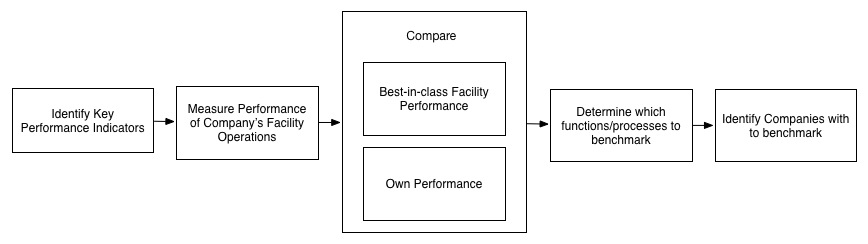
\includegraphics[width=1.1\textwidth]{img/IFMAMethBenchProcess.jpg}
  \end{adjustwidth}
  \caption{IFMA Benchmarking Methodology adapted from Roka-Madarasz \cite{Roka-Madarasz2010}. First step is to identify the KPI, then, use it to measure the facility performance. At this point three different paths can be taken: Best-in-class Facility Performance, Own Performance, or directly to Compare. After this, the functions of benchmark has to be chosen, just like which companies to benchmark.}
  \label{fig:IFMAMethodology}
\end{figure}

In order to measure facilities performance, IFMA has established 9 Key Performance Indicators that must be easily measurable and that must be defined for monitoring the actual process and also to control it. These Key Performance Indicators shown in the report \cite{Roka-Madarasz2010} can be seen in Table \ref{tb:TableKPIFMBenchmarking} on Appendix.

% \subsubsection{BOMA}

% \hfill \\ \\ The Building Owners and Managers Association (BOMA International) is a organization for commercial real estate professionals such as building owners, managers, developers, leasing professional, products and services providers, etc. It is a federation of 93 BOMA U.S. associations, BOMA Canada and its 11 regional associations and 13 BOMA international affiliates.

% Its objective is to advance the interests of the entire commercial real estate industry through advocacy, education, research, standards and information, so, BOMA monitor and lobby pertinent legislative, regulatory and codes/standards issues (electricity deregulation, capital gains tax relief, telecommunications, indoor air quality, etc). 

% BOMA International is a primary source of information on building management and operations, development, leasing, building operating costs, energy consumption patterns, local and national building codes, legislation, occupancy statistics, technological developments and other industry trends.

\subsection{Existing Solutions}

As specified in section \ref{FacilitiesManagement}, there are many types of softwares for FM solutions, like CAFM or IWMS. All of known FM solutions like Maxpanda \cite{maxpanda} or IBM Tririga \cite{IBMtririga} are a simpler way to manage facilities, they centralize organizations information, making management more efficient through business analytics, critical alert, increasing visibility and control.

Some of them, like ARCHIBUS \cite{ARCHIBUSsite} or FM:Systems \cite{FMsystems} have integration with CAD or BIM models, which is very important for visualization of departments occupation or others space and occupation management areas. 

Most of these systems promotes their capabilities for organizations cost reduction --- since they cost-justify real changes in preventive maintenance routines and predicts cost effects of preventive maintenance changes before they are made --- some permits multiple users, others make possible that each user only can access specific information regarding his organization position.

There are different sectors that a FM system can focus like 
\begin{enumerate*}[label=\itshape\roman{enumi})]
	\item Capital/ Financial,
	\item Real Estate/Retail: Construction or Project Management,
	\item Space and Workplace, 
	\item Maintenance, 
	\item Sustainability and Energy,
	%\item Document, 
	\item Move,
	%\item Facilities,
	\item Higher Education and Public 
\end{enumerate*}. Many of the existent solutions only focus in some of this sectors and not in all of them.

For Real Estate it is usual features for incorporation of current lease accounting standards, tracking of dates and contractual commitments, management of occupancy and facilities costs. 
On Capital/Finantial are being used features to identify funding priorities within capital programs, reduce project schedule overruns or streamline project cost accounting.
In Space and Workplace it is important to have tools for space use agreements and chargeback to increase departmental accountability for space use.
Maintenance requires features for automatically route and manage both incoming and planned maintenance, while at the same time keeping internal customers up to date on the progress of their work tickets, or streamline facility maintenance, service management and facility condition assessments. 
The Sustainability and Energy sector is also very important for defining which projects will achieve the right mix of environmental benefits and cost savings, for reduce energy consumption to meet sustainability goals, identifying poorly performing facilities and automate corrective actions.

Systems like Indus System \cite{IndusSystems}, Manhattan Mobile Apps \cite{ManhattanAppMobile}, PNMSoft \cite{pnmSoftsite} or ARCHIBUS have cloud-based software that enables users to access FM systems anywhere on mobile devices from a browser.
Indus System enables users to store, share, view drawings, space, assets, related costs, leases and contracts just by accessing the browser.

For other hand, ARCHIBUS and PNMSoft are both capable of showing an organizations KPIs through their web site. The packages enables users normal usage of their daily management software and then, when necessary, the visualization of the results on a graphical web application.
However, this solution is only applicable for the facilities that have ARCHIBUS or PNMSoft software installed, and only for comparison from previous results from that facility.
In contrast, with our solution, any organization could benefit from this features and one more: the comparison with others organizations on the sector.

\subsubsection{ARCHIBUS}

\hfill \\ \\ ARCHIBUS is the provider Facilities Management software solution that effectively tracks and analyzes not only facilities-related information but also real-estate. ARCHIBUS is an integrated solution that applies to organizations of all sizes and sectors (here we focus on ARCHIBUS for Educational Institutions reports - Table \ref{tb:ARCHIBUSListActReports} on Appendix).

The system architecture consists of three main modules (as seen on Figure \ref{fig:ArchiModules}), the first, is named ARCHIBUS Web Central and provides live enterprise access to facilities data and enables the easy maintenance and distribution of facilities information across the entire enterprise \cite{ARCHI}. A role-based security service, allows that when users log on, they only access information relevant to their roles on the organization.

\begin{figure}[t!]
  \centering
  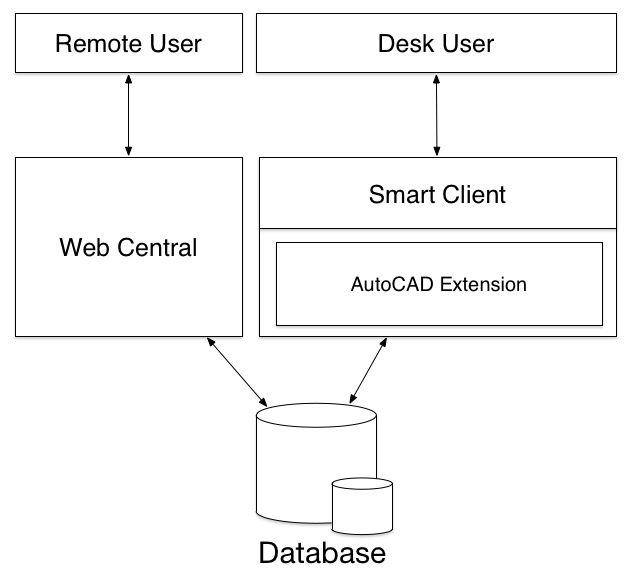
\includegraphics[width=0.50\textwidth]{img/ARCHIBUSModules.jpg}
  \caption{Overview of ARCHIBUS software architecture adapted from ARCHIBUS Fundamentals Training \cite{ARCHI}. The Database is the same for all modules, so the data is coherent between them. Module Extension for AutoCAD is only applicable for the module Smart Client, that can only be used by Desk Users. Remote users that are not on the office, can use Web Central to access data.}
  \label{fig:ArchiModules}
\end{figure}
 
ARCHIBUS have a .NET Windows application, named Smart Client, used by back-office personnel for data entry, data transfer, importing and exporting data from other systems. This module has another one integrated, the Smart Client Extension for AutoCAD or DWG Editor that is very important for those organizations who want to include Computer-Aided Drawing or BIM models.  

From a technical standpoint, the software architecture of ARCHIBUS consists of a database that can be one of MS SQL, Oracle or Sybase. This database communicates with the application servers that can run on Tomcat, Jetty, WebLogic or WebSphere. The applications of SmarClient module running on the computer of the client companies, communicate with application servers through Web Services and the applications of Web Central module communicates via HTTP with those same servers \cite{ARCHI}.

Being part of the ARCHIBUS platform, ARCHIBUS Performance Metrics Framework delivers KPIs and other performance data about the real estate, infrastructure and facilities using a detailed graphical view of the data. Thus, it is possible to use analytical measures and productivity tools, which provides decision-makers to align their portfolio to organizational strategy, spotlight underperforming business units or assets, and benchmark organizational progress to achieve targeted goals.

\subsubsection{PNM Soft Sequence Kinetics}

\hfill \\ \\ PNM Soft Sequence Kinetics is an Intelligent Business Process Management Suite and covers process optimizing KPI, dynamic process change, KPI analysis, process operation and tracking, communication with external systems and mobile and cloud KPI.

This system has four main focus: Processing-Optimizing KPI, Process Operation and Visual Tracking, KPI for Process Administrators and Mobile Process KPI.

On the Process Optimizing KPI there are two different processes: 
\begin{description}
	\item  [Extra-Process Performance Analytics] permits the process performance tracking via runtime dashboards and displays KPI like process status levels or average execution time of a process, which helps to understand how successful the process is and highlight required improvement areas.\\

	\item  [Intra-Process Analytics] aggregation and calculation of intra-process data by real-time analytics, that is built into the Business Rule editor, which enables routing according to their results via a simple GUI, being an artificial process intelligence form which sees the business teach itself how to perform better over time.
\end{description}

Process Operation and Visual Tracking is possible by Flowtime that is a extension of Microsoft SharePoint with a built-in process operation environment, which enables the collaboration on processes in a familiar interface and includes advanced task management, delegation and monitoring of KPI capabilities with a tracking views, which shows the process stands.

The KPI for Process Administrators provides important indicators on process performance per type of process \cite{PNMSOFT}.

PNM Soft also has a mobile application named Mobile Portal, that is available as an application or an online service, where users can access the same features provided by Sequence Kinetics Flowtime and can be configured by the customer to meet his necessities. 
For the cloud platform PNM Soft uses Windows Azure.

\subsection{Scientific Literature} \label{ScientificStudies}

Ho et al \cite{Ho2000} report different performance measurements and indicators most used in Asia Pacific region. This research work rates the importance of 97 metrics on a five point scale and indicate if the metric was being used in their organization FM --- the metrics consisted of performance measurements and performance indicators grouped by eight categories:
\begin{enumerate*}[label=\itshape\roman{enumi})]
 	\item size and use of facilities,
 	\item maintenance,
 	\item refurbishment,
 	\item cleaning,
 	\item energy consumption,
 	\item ground and environment,
 	\item safety and security,
 	\item parking.
\end{enumerate*}
These categories are represented by order of importance on Figure \ref{fig:MeasurementCatPriority}, according to the study by Ho et al \cite{Ho2000}.
% \begin{table}
% 	\begin{adjustwidth}{4,5cm}{0cm}
% 	\begin{tabular}{l}
% 		\multicolumn{1}{c}{\bf Category} \\
% 		\hline
% 		Cleaning \\
% 		Refurbishment \\
% 		Parking \\
% 		Ground and Environment \\
% 		Size and use of facilities \\
% 		Safety and Security \\
% 		Maintenance \\
% 		Energy Consumption \\	
% 		\hline
% 	\end{tabular}
% 	\end{adjustwidth}
% \caption{Measurement Categories ordered by their importance according to the results of the research of Ho et al \cite{Ho2000}.}
% \label{tb:CategoriesHo}
% \end{table}

\begin{figure}[t!]
  \centering
  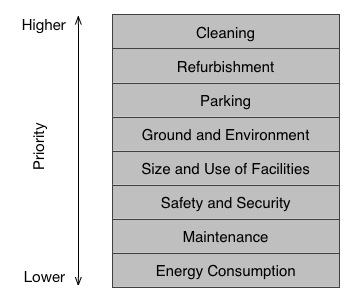
\includegraphics[width=0.40\textwidth]{img/MeasurementCatPriority.jpg}
  \caption{Measurement Categories ordered by their importance according to the results of the research of Ho et al \cite{Ho2000}.}
  \label{fig:MeasurementCatPriority}
\end{figure}



Moreover, Ho et al \cite{Ho2000} also identified which of the 97 metrics were the most used and more important to the organizations: the metrics that lead a direct financial implication were the ones with a higher rating. The 30 metrics with higher rates are especially related to the areas of:
\begin{enumerate*}[label=\itshape\roman{enumi})]
 	\item Financial such as Total Annual Facility Cost and Operational Cost, 
 	\item Spacial such as Gross Floor Area/Usable Floor Area and Usable Area,
 	\item Maintenance such as Asset Replacement Value (Maintained),
 	\item Cleaning such as Area Cleaned and Cleanliness Status of Site.
\end{enumerate*}

% \begin{enumerate*}[label=\roman{enumi})]
% 	\item Total Annual Facility Cost,\\
% 	\item Total Maintenance Expenditure,\\
% 	\item Total Cleaning Cost,\\
% 	\item Initial Cost,\\
% 	\item Operation Cost,\\
% 	\item Cleaning Expenditure/m2,\\
% 	\item Total Refurbishment Value (total),\\
% 	\item Annual Income,\\
% 	\item Gross Floor Area/Usable Floor Area,\\
% 	\item Cleanliness Status of Site, Interior and Exterior and Fittings, etc,\\
% 	\item Annual Consumption,\\
% 	\item Gross Floor Area,\\
% 	\item Competence of in-house staff,\\
% 	\item Adequacy of Budget,\\
% 	\item Annual Cost of Energy Purchased,\\
% 	\item Total Number of Parking Spaces Available,\\
% 	\item Usable Area,\\
% 	\item Rentable Area,\\
% 	\item Operation Cost/m2,\\
% 	\item Occupants Satisfaction,\\
% 	\item Frequency of Building Failures,\\
% 	\item Facility Budget/Corporation Budget,\\
% 	\item Asset Replacement Value (Maintained),\\
% 	\item Cost per m2,\\
% 	\item Total ground Maintenance Expenditure,\\
% 	\item Total Environment Cost,\\
% 	\item Occupancy Cost/m2,\\
% 	\item Facility Budget/Facility Assets,\\
% 	\item Area Cleaned.
% \end{enumerate*}

Massheder and Finch \cite{Mass1998}, surveyed the FM benchmarking metrics used in the UK. Their work identified which metrics were used to measure performance of the FM function. They organized metrics according to five categories:
\begin{enumerate*}[label=\itshape\roman{enumi})]
	\item business metrics,
	\item building performance metrics,
	\item portfolio metrics,
	\item acquisition  metrics,
	\item disposal metrics. 
\end{enumerate*} The results of their study are presented in Table \ref{tb:TableUseBenchmarkingMetrics}. As we can see, the most used metrics are the Business, Portfolio Metrics and Building Performance. The latter is considered the most important one (with percentage of use above 50\% on 5 of 6 metrics presented.)

\begin{table}[h!]
	\vspace{0cm}
	\begin{adjustwidth}{-0,5cm}{0cm}
	\begin{tabular}{l r}
		\hline
		\multicolumn{1}{l}{\bf Metric} & \multicolumn{1}{r}{ \bf Percentage of Use } \\ 
		\hline

		{\bf {\emph{Business}}} & \\
		Occupancy cost of operating revenue by building &  43\% \\
		Occupancy cost of the total of labour and costs by business unit &  29\% \\
		Occupancy of cost of operating revenue by business unit &  21\% \\ 
		Occupancy cost of the total sales and admin cost by business unit  &  14\% \\ 
		Location analysis on basis of where key skills are available & 7\% \\ 
		Location optimization (in context of attractors and repellers) &  7\% \\ 
		\hline

		{\bf {\emph{Building Performance}}} & \\
		Occupancy cost per $m^2$ &  98\% \\
		Occupancy cost per person &  79\% \\
		Occupancy of cost per building size &  64\% \\ 
		$m^2$ per person  &  64\% \\ 
		Itemized (occupancy) cost comparisons of $m^2$ per person by building & 36\% \\ 
		Absentee rates by building &  0\% \\ 
		\hline

		{\bf {\emph{Portfolio Metrics}}} & \\
		Proportion of operational space compared to non-operational space &  49\% \\
		Current market capital value compared to book value by building &  21\% \\
		Current market rental value compared to rent peasing by building &  14\% \\ 
		Proportion of Non-operational Space that is Sublet or Assigned  &  14\% \\ 
		\hline

		{\bf {\emph{Acquisition Metrics (only those who include real estate in FM)}}} & \\
		Costs of acquisition measured against returns &  20\% \\
		Actual extra occupancy cost against prediction cost &  10\% \\
		Amount of space coming on stream per unit time &  10\% \\ 
		Time to find and acquire space against program &  10\% \\ 
		Time to occupation against program & 10\% \\ 
		\hline

		{\bf {\emph{Disposal Metrics (only those who include real Estate in FM)}}} & \\
		Holding costs per year &  30\% \\
		 Time to dispose of buildings against program &  30\% \\
		 Cost of disposal against savings &  20\% \\ 
		Time to clear buildings against program  &  20\% \\ 
		 Holding costs to lease end, break and/or estimated disposal date & 10\% \\ 
		 Number of months vacant to date &  10\% \\ 
		 Disposal performance measures against natural portfolio shed rate & 0\% \\ 
		 Months vacancy to lease end, break and/or estimated disposal date &  0\% \\ 
		\hline

	\end{tabular}
	\end{adjustwidth}
\caption{Use of the different metrics on UK benchmarking organizations according to Massheder et al \cite{Mass1998}. The most used metrics are the ones belonging to Building Performance, Business and Portfolio with a percentage of use above the Acquisition and Disposal categories.}
\label{tb:TableUseBenchmarkingMetrics}
\end{table}

%Gilleard and Yat-lung (2004) suggested applying Analytic Hierarchy Process (AHP) to FM benchmarking. AHP, designed in 1970 by Saaty, helps decision-makers set priorities and make best decision when both qualitative and quantitative aspects of decision need to be considered, making complex problems into small ones \cite{Gilleard2004}.
%After their study, they arrived at a conclusion that applying AHP to FM benchmarking helps facility managers to assimilate all the facts, weight the pros and cons and communicate the performance benchmarks in a logical manner \cite{Gilleard2004}.


Hinks and McNay \cite{Hinks1999} identified a need to established a set of universally accepted KPI that realistically evaluate organizations performance.  
On their study, they identified the need to clarify and prioritize the parameters and indicators which correlated the views of the customer and the departments, to support the operational requirements of the core financial business. To this end, they used the Delphie technique \cite{Eynde1997} (used to gather expert opinion in areas where there is considerable uncertainty and/or lack of agreed knowledge \cite{Hinks1999}), where a group of the premises department and their internal customers were consulted using questionnaires, scenario workshops and group discussions set.

The first phase of Hinks and McNay's study consisted of a literature review, where the authors concluded that the practical use of KPIs frequently involves industry-specific or organization-specific indicators. They also concluded that most of the indicators were providing data that were of direct applicability for monitoring the management of FM tasks. Unfortunately these indicators were not likely to be relevant to their customers \cite{Hinks1999}. 
Since no single measure can adequately provide a clear performance target, it is desirable a balance between financial and non-financial measures \cite{Slater1997}. Taking this into account, were chosen 172 KPIs that can be consulted on Hinks paper \cite{Hinks1999}, also, performance indicators must be comparable and sufficiently complete and objective to accurately describe the address FM function \cite{Wang1992}.

The study had a second phase where the group of responders were asked to prioritize the performance parameters from the previous KPI list, selecting a comprehensive and coherent set (they could also add indicators if they though best). At the end, the group choose 23 KPIs as the most representative of the study.
On phase three, it was allocated a grade, between 0 and 10, for each KPI, according to its importance. Less that 4 indicated that the indicator was only of minimal relevance, a mark between 4 and 7 (inclusive) indicated increasing levels of importance, and a mark which exceeded 7 identified a supremely important indicator of FM performance \cite{Hinks1999}. The list can be found on Table \ref{tb:23KPIimportanceOrder}.

\begin{table}[h!]
	%\vspace{0cm}
	\begin{adjustwidth}{0,2cm}{0cm}
	\begin{tabular}{r l c}
		\hline
		\multicolumn{1}{ c }{\bf Performance Dimension} &  \multicolumn{1}{c }{\bf Metric} \\ 
		\hline

		\multicolumn{1}{  l  }{\multirow{1}{*}{\bf {\emph{Business}}}} &  No loss of business due to failure of premises services \\
		\multicolumn{1}{  l  }{\multirow{1}{*}{\bf {\emph{General}}}} &  Customer Satisfaction \\
		\multicolumn{1}{  l  }{\multirow{1}{*}{\bf {\emph{Change Management}}}} &  Completion of project to customer satisfaction \\
		\multicolumn{1}{  l  }{\multirow{1}{*}{\bf {\emph{Environment}}}} &  Provision of safe environment\\
		\multicolumn{1}{  l  }{\multirow{1}{*}{\bf {\emph{Space}}}} &  Effective utilization of space \\
		\multicolumn{1}{  l  }{\multirow{1}{*}{\bf {\emph{Change Management}}}} &  Effectiveness of communication \\
		\multicolumn{1}{  l  }{\multirow{1}{*}{\bf {\emph{Maintenance}}}} &  Reliability \\
		\multicolumn{1}{  l  }{\multirow{1}{*}{\bf {\emph{General}}}} &  Professional approach of premises staff \\
		\multicolumn{1}{  l  }{\multirow{1}{*}{\bf {\emph{General}}}} &  Responsiveness to problems \\
		\multicolumn{1}{  l  }{\multirow{1}{*}{\bf {\emph{General}}}} & Competence of staff \\
		\multicolumn{1}{  l  }{\multirow{1}{*}{\bf {\emph{Maintenance}}}} & Management of maintenance \\
		\multicolumn{1}{  l  }{\multirow{1}{*}{\bf {\emph{Change Management}}}} & Responsiveness of PD to changes/requirements \\
		\multicolumn{1}{  l  }{\multirow{1}{*}{\bf {\emph{Business}}}} &  Value for money \\
		\multicolumn{1}{  l  }{\multirow{1}{*}{\bf {\emph{Environment}}}} &  Satisfactory physical working conditions \\
		\multicolumn{1}{  l  }{\multirow{1}{*}{\bf {\emph{Equipment}}}} &  Equipment provided meets business needs \\
		\multicolumn{1}{  l  }{\multirow{1}{*}{\bf {\emph{Business}}}} &  Suitability of premises and functional environment \\
		\multicolumn{1}{  l  }{\multirow{1}{*}{\bf {\emph{Change Management}}}} &  Quality of end product \\
		\multicolumn{1}{  l  }{\multirow{1}{*}{\bf {\emph{Maintenance}}}} &  Effectiveness of helpdesk service \\
		\multicolumn{1}{  l  }{\multirow{1}{*}{\bf {\emph{Change Management}}}} &  Achievement of completion deadlines \\
		\multicolumn{1}{  l  }{\multirow{1}{*}{\bf {\emph{Equipment}}}} & Correction of faults \\
		\multicolumn{1}{  l  }{\multirow{1}{*}{\bf {\emph{Maintenance}}}} &  Standards of cleaning \\
		\multicolumn{1}{  l  }{\multirow{1}{*}{\bf {\emph{General}}}} &  Management information \\
		\multicolumn{1}{  l  }{\multirow{1}{*}{\bf {\emph{Environment}}}} &  Energy performance \\
		\hline


	\end{tabular}
	\end{adjustwidth}
\caption{The final list of 23 KPIs to support operational requirements of organizations, ordered by importance according to Hinks et al \cite{Hinks1999}. Higher importance indicators come at the top.}
\label{tb:23KPIimportanceOrder}
\end{table}

In 2004, Costa et al \cite{Costa2004}, made a discussion about three benchmarking initiatives in United Kingdom (Key Performance Indicators Working Group, 2000), United States of America (Construction Industry Institute, 2000) and Chile (Corporacion de Desarrolo Tecnológico, 2002). They described two projects that aimed to conceive and implement performance measurement systems for benchmarking in the Brazilian construction industry.

The objective of the initiatives mentioned previously was to measure the performance of the FM sector, and to identify and evaluate best practices, through comparison of key performance indicators. To this end, a web-based online tool was developed, enabling to input previously gathered data. Tools were provided for displaying graphically the comparative performance of companies involved.

Each one of the studies considered by Costa et al selected the KPIs by combining distinct approaches: extensive reviews by a panel of experts and the publication of an initial report, selection based on previous studies, or by a committee involving both industry representatives and Construction Industry Institute.

Performance measurements as cost, safety and time were common between the studies. The resume of those systems (including the Costa et al final solution) KPI selections were essentially focused on categories such as Financial (Deviation of Cost by Project), Safety (Labor Accident Rate), Satisfaction (Client and Employee) and Performance (Project Schedule Growth).
Based on the experience of these surveys, the authors also concluded that the set of measures should 
\begin{enumerate*}[label=\roman{enumi})]
	\item be simple and 
	\item well designed in order to support improvement, and 
	\item give a comprehensive company wide-view \cite{Costa2004}. 
\end{enumerate*} 
% \begin{enumerate*}[label=\roman{enumi})]
% 	\item Client satisfaction,\\
% 	\item Defects,\\
% 	\item Predictability Cost,\\
% 	\item Predictability Time,\\
% 	\item Profitability,\\
% 	\item Safety,\\
% 	\item Productivity Performance,\\
% 	\item Deviation of Cost by Project,\\	 
% 	\item Deviation of Time by Project,	\\		
% 	\item Deviation of Construction Due Date,\\
% 	\item Change in Amount Contracted,\\
% 	\item Rate of Subcontract,\\
% 	\item Cost Client Complaints,\\
% 	\item Efficiency of Direct,\\
% 	\item Labor Accident Rate,\\
% 	\item Risk Rate (Ratio between the number of accidents and total man-hour input),\\
% 	\item Effectiveness of Planning (Percentage of Plan Completed),\\
% 	\item Urgent Orders,\\
% 	\item Project Cost Growth,\\
% 	\item Project Budget Factor,\\
% 	\item Project Schedule Growth,\\
% 	\item Project Schedule Factor,\\
% 	\item Total Project Duration,\\
% 	\item Change Cost Factor,\\
% 	\item Recordable Incident Rate (RIR),\\
% 	\item Lost Workday Case Incident Rate (LWCIR),\\
% 	\item Total Field Rework,\\
% 	\item Factor Phase Cost,\\
% 	\item Factor Phase Cost Growth,\\ 
% 	\item Phase Duration Factor,\\
% 	\item Average Time for Selling Units,\\
% 	\item Contracting Index,\\
% 	\item Supplier performance,\\
% 	\item Construction Site Best Practice Index,\\
% 	\item Non-Conformity Index in the unit delivery,\\
% 	\item Number of Non-Conformity in audit,\\
% 	\item Degree of employee Satisfaction,\\
% 	\item Training Index,\\
% 	\item Construction Phase Duration.
% \end{enumerate*} 

Costa et al \cite{Costa2005} took the investigation further, and in 2005 they developed an online benchmarking application which offers analysis and simulation of organizations performance with respect to reference values found for each sector. 
The data being reported is related to reference values and general results, keeping confidential information from companies participating in the project.
%Organizations can access the site through a login form where the administrator will have the data control and can give access to six more users responsible for the data insertion. The system also permits the printing of indicators worksheets and generate reports with company data and compare it with reference values of the participating companies.

 

%\subsection{Appraisal}



\subsection{Discussion}

The problem of KPIs identification in the domain of FM had already been studied by distinct system industries and scientific studies. However, there is not any accorded standardization or prioritization used by the industry. The determination of which KPIs to use for a centralized benchmarking infrastructure for FM is still an open question.  
In order to understand what are the most relevant KPIs for the field of FM we combined the results of distinct authors.
Table \ref{tb:ListSpacialFinancialKPIpapers} presents the various KPIs pointed out by the scientific literature along with the frequency of reference. Through it, is possible to identify which ones are the most referenced, and which, on a theoretical level, correspond to the ones that should be used on this project solution. 

KPIs are performance measurements, thus, it is indispensable to normalize them and specify how they can be achieved.
Table \ref{tb:ListSpacialFinancialHowCalculate} describes how each one of the previous KPIs can be calculated. Indicators on categories such as Quality and Satisfaction have to be measured through audits or questionnaires (an example of Quality of Cleaning questionnaires can be seen on tables \ref{tb:RoutineCleaningQuesitonnarie} and \ref{tb:SpecialCleaningQuesitonnarie} on Appendix).

%Through the  previous scientific literature it was possible to make a systematization of the different indicators. However, it was difficult to achieve a coherent list of KPIs since the authors gave distinctive names for correspondent indicators. Thus, it was necessary a convergence of the various indicators presented in the diverse studies. The result can be consulted in Tables \ref{tb:ListSpacialFinancialKPIpapers} and \ref{tb:Resto2ListKPIpapers}.
%Analyzing the information on them, it was possible to conclude that the most used categories are Financial and Space Indicators. In each category there are most used Indicators that are systematized on Table \ref{tb:ListFinalKPI}, and that corresponds to the KPIs that will be used on the solution proposed by this document.
%Combining these most used indicators, to some indicators that,
%Can also be seen on Table \ref{tb:ListSpacialFinancialHowCalculate} and \ref{tb:Resto2ListHowCalculate} the measurements necessaries for each KPI. Some cases the measurement for a KPI is not a formula but a measure obtained trough questionnaires or audits. An example of this case is the Quality of Cleaning. On Tables \ref{tb:RoutineCleaningQuesitonnarie} and \ref{tb:SpecialCleaningQuesitonnarie} can be seen an example of these questionnaires.

\begin{table}%[t!]
	\vspace{-1,5cm}
	\begin{adjustwidth}{2cm}{0cm}
	\resizebox{8cm}{!} {
	\begin{tabular}{p{6cm}llllllp{1cm}lr}
		\hline
		 {\bf Indicators} &  \begin{sideways}{\bf Costa et. al \cite{Costa2004}}\end{sideways} & \begin{sideways}{\bf USA, UK and Chile Projects \cite{Costa2004}}\end{sideways} & \begin{sideways}{\bf IFMA \cite{Roka-Madarasz2010}}\end{sideways} & \begin{sideways}{\bf ARCHIBUS}\end{sideways} & \begin{sideways}{\bf Ho et. al \cite{Ho2000}}\end{sideways} & \begin{sideways}{\bf Massheder et. al \cite{Mass1998}}\end{sideways} & \begin{sideways}{\bf Hinks et. al \cite{Hinks1999}}\end{sideways} & {\bf Total} \\ 

		\hline
		{\bf Financial Indicators} 	& & & & & & & & \\
		Total Cleaning Cost 				& & &$\bullet$ & & & & & 1 \\
		Cleaning Cost per $m^2$ 			& & &$\bullet$ &$\bullet$ & & & & 2 \\
		Total Maintenance Cost 				& & &$\bullet$ &$\bullet$ &$\bullet$ & & & 3 \\
		%Janitorial Costs 					& & & & &$\bullet$ & & & 1 \\
		FM Costs 							& & & &$\bullet$ & & & & 1 \\
		Utility Costs 						& & & & &$\bullet$ & & & 1 \\
		Facility Budget/Corporation Budget 	& & &$\bullet$ & & & & & 1 \\
		Occupancy Cost per $m^2$ 			& & &$\bullet$ & &$\bullet$ &$\bullet$ & & 3 \\
		Space Costs per $m^2$ 				& & &$\bullet$ &$\bullet$ &$\bullet$ & & & 3 \\
		%ICT Costs 							& & & &$\bullet$ & & & & 1 \\
		%Adequacy of Budget 					& & &$\bullet$ & & & &$\bullet$ & 2 \\
		Operation Cost per $m^2$ 			& & &$\bullet$ &$\bullet$ & &$\bullet$ & & 3 \\
		%Business Support Costs 				& & & &$\bullet$ & & & & 1 \\
		Moving Costs 						& & & & &$\bullet$ & & & 1 \\
		%Workplace Costs 					& & & & &$\bullet$ & & & 1 \\
		%Space Planning Costs 				& & & & &$\bullet$ & & & 1 \\
		HSSE Costs 							& & & &$\bullet$ &$\bullet$ & & & 2 \\
		Security Costs 						& & & & &$\bullet$ & & & 1 \\
		%Life-safety Costs 					& & & & &$\bullet$ & & & 1 \\
		Logistic Costs 						& & & &$\bullet$ & & & & 1 \\
		Hospitality Costs 					& & & &$\bullet$ & & & & 1 \\
		Project Costs (Deviation) 			&$\bullet$ &$\bullet$ & & &$\bullet$ & &$\bullet$ & 4 \\
		Financial Ratios 					& &$\bullet$ & & &$\bullet$ & &$\bullet$ & 3 \\
		Annual Income 						& & &$\bullet$ & & & &$\bullet$ & 2 \\
		Total Annual Facility Cost 			& & &$\bullet$ & &$\bullet$ &$\bullet$ & & 3 \\
		Annual Cost of Energy Purchased 	& & &$\bullet$ & & & & & 1 \\
		Total Environment Cost 				& & &$\bullet$ & &$\bullet$ & & & 2 \\
		Outdoor Costs 						& & & & &$\bullet$ & & & 1 \\
		\hline
		{\bf Spacial Indicators}	& & & & & & & & \\
		Net Floor Area 						& & &$\bullet$ &$\bullet$ &$\bullet$ &$\bullet$ &$\bullet$ & 5  \\
		Percentage Net Floor Area 			& & &$\bullet$ &$\bullet$ &$\bullet$ & &$\bullet$ & 4 \\
		Percentage Internal Area			& & &$\bullet$ &$\bullet$ &$\bullet$ & &$\bullet$ & 4 \\
		Percentage Gross Floor Area 		& & &$\bullet$ &$\bullet$ &$\bullet$ & &$\bullet$ & 4 \\
		Support Area 						& & & & &$\bullet$ & & & 1 \\
		\hline
		{\bf Maintenance/Cleaning Indicators}							& & & & & & & & \\
		Repairs VS Preventive Maintenance 										& & & & &$\bullet$ & &$\bullet$ & 2 \\
		%Outworking of Maintenance 												& & & & &$\bullet$ & &$\bullet$ & 2  \\
		Asset Replacement Values												& & &$\bullet$ & & & &$\bullet$ & 2 \\
		Percentage of Area Cleaned			 									& & &$\bullet$ & & & &$\bullet$ & 2 \\
		\hline
		{\bf Productivity Indicators} & & & & & & & & \\
		Core operating hours of facility (FM) 		& & & &$\bullet$ & & & & 1 \\
		%Timeless of Service provision (FM) 			& & & &$\bullet$ & & & & 1 \\
		Uptime Facility (Business)					& & & &$\bullet$ & & & & 1 \\
		%Recovery Time (Business) 					& & & &$\bullet$ & & & & 1 \\
		Staff Turnover (Human Resources) 			& & & &$\bullet$ & & &$\bullet$ & 2 \\
		Absenteeism (Human Resources) 				& & & &$\bullet$ & & &$\bullet$ & 2 \\
		\hline
		{\bf Environmental Indicators} & & & & & & & & \\
		CO2 emissions 						& & & &$\bullet$ & & & & 1 \\
		Total Energy Consumption 	 		& & & &$\bullet$ & & &$\bullet$ & 2 \\
		Total Water Usage					& & & &$\bullet$ & & & & 1 \\
		Total Waste Production 				& & & &$\bullet$ & & & & 1 \\
		%Space and Environment 				& & & &$\bullet$ & & & & 1 \\
		%Outdoors and Environment 			& & & &$\bullet$ & & & & 1 \\
		%Workplace and environment 			& & & &$\bullet$ & & &$\bullet$ & 2 \\
		%Utilities and environment 			& & & &$\bullet$ & & &$\bullet$ & 2 \\
		%Health and safety and environment 	& & & &$\bullet$ & & &$\bullet$ & 2 \\
		%Mobility and environment 			& & & &$\bullet$ & & & & 1 \\
		%Procurement and environment 		& & & &$\bullet$ & & & & 1 \\
		\hline
		{\bf Service Quality Indicators} & & & & & & & & \\
		Quality of Product 							& &$\bullet$ & & & & &$\bullet$ & 2 \\
		%Quality of Facility Management 				& & & &$\bullet$ & & &$\bullet$ & 2 \\
		Quality of Cleaning							& & & &$\bullet$ & & &$\bullet$ & 2 \\
		Quality of Workplace 						& & & &$\bullet$ & & &$\bullet$ & 2 \\
		Quality of Security 						& & & &$\bullet$ & & &$\bullet$ & 2 \\
		Quality of Reception and Contact Center 	& & & &$\bullet$ & & & & 1 \\
		%Quality of Catering and Vending				& & & &$\bullet$ & & &$\bullet$ & 2 \\
		Quality of Document Management 				& & & &$\bullet$ & & & & 1 \\
		\hline
		{\bf Satisfaction Indicators} & & & & & & & & \\ 
		Client Satisfaction 			&$\bullet$ &$\bullet$ & & & & &$\bullet$ & 3  \\
		Satisfaction with FM 			& & & &$\bullet$ & & & & 1 \\
		Satisfaction with Space			& & & &$\bullet$ & & & & 1 \\
		Satisfaction with Outdoors 		& & & &$\bullet$ & & & & 1 \\
		Satisfaction with Cleaning 		& & & &$\bullet$ & & & & 1 \\
		Satisfaction with Workspace 	& & & &$\bullet$ & & & & 1 \\
		Satisfaction with HSSE			& &$\bullet$ & &$\bullet$ & & & & 2 \\
		Satisfaction with Hospitality	& & & &$\bullet$ & & & & 1 \\
		Satisfaction with ICT 			& & & &$\bullet$ & & & & 1 \\
		Satisfaction with Logistics 	& & & &$\bullet$ & & & & 1 \\
	\end{tabular}
	}
	\end{adjustwidth}
\caption{List of KPIs covered by the literature. It is represented the various KPIs referred by the scientific literature. On the last column, it is represented the total of documents that referred that specific KPI.}
\label{tb:ListSpacialFinancialKPIpapers}
\end{table}

% \begin{table}[h!]
% 	\vspace{-3cm}
% 	\begin{adjustwidth}{1cm}{0cm}
% 	\begin{tabular}{p{6cm}llllllp{1cm}lr}
% 		\hline
% 		 {\bf Indicators} &  \begin{sideways}{\bf Costa et. al \cite{Costa2004}}\end{sideways} & \begin{sideways}{\bf USA, UK and Chile Projects \cite{Costa2004}}\end{sideways} & \begin{sideways}{\bf IFMA \cite{Roka-Madarasz2010}}\end{sideways} & \begin{sideways}{\bf ARCHIBUS}\end{sideways} & \begin{sideways}{\bf Ho et. al \cite{Ho2000}}\end{sideways} & \begin{sideways}{\bf Massheder et. al \cite{Mass1998}}\end{sideways} & \begin{sideways}{\bf Hinks et. al \cite{Hinks1999}}\end{sideways} & {\bf Total}\\ 
% 		\hline
% 		{\bf Maintenance/Cleaning Indicators}							& & & & & & & & \\
% 		Repairs VS Preventive Maintenance 										& & & & &$\bullet$ & &$\bullet$ & 2 \\
% 		%Outworking of Maintenance 												& & & & &$\bullet$ & &$\bullet$ & 2  \\
% 		Asset Replacement Values												& & &$\bullet$ & & & & & 1 \\
% 		Percentage of Area Cleaned			 									& & &$\bullet$ & & & &$\bullet$ & 2 \\
% 		\hline
% 		{\bf Productivity Indicators} & & & & & & & & \\
% 		Core operating hours of facility (FM) 		& & & &$\bullet$ & & & & 1 \\
% 		%Timeless of Service provision (FM) 			& & & &$\bullet$ & & & & 1 \\
% 		Uptime Facility (Business)					& & & &$\bullet$ & & & & 1 \\
% 		%Recovery Time (Business) 					& & & &$\bullet$ & & & & 1 \\
% 		Staff Turnover (Human Resources) 			& & & &$\bullet$ & & &$\bullet$ & 2 \\
% 		Absenteeism (Human Resources) 				& & & &$\bullet$ & & &$\bullet$ & 2 \\
% 		\hline
% 		{\bf Environmental Indicators} & & & & & & & & \\
% 		CO2 emissions 						& & & &$\bullet$ & & & & 1 \\
% 		Total Energy Consumption 	 		& & & &$\bullet$ & & &$\bullet$ & 2 \\
% 		Total Water Usage					& & & &$\bullet$ & & & & 1 \\
% 		Total Waste Production 				& & & &$\bullet$ & & & & 1 \\
% 		%Space and Environment 				& & & &$\bullet$ & & & & 1 \\
% 		%Outdoors and Environment 			& & & &$\bullet$ & & & & 1 \\
% 		%Workplace and environment 			& & & &$\bullet$ & & &$\bullet$ & 2 \\
% 		%Utilities and environment 			& & & &$\bullet$ & & &$\bullet$ & 2 \\
% 		%Health and safety and environment 	& & & &$\bullet$ & & &$\bullet$ & 2 \\
% 		%Mobility and environment 			& & & &$\bullet$ & & & & 1 \\
% 		%Procurement and environment 		& & & &$\bullet$ & & & & 1 \\
% 		\hline
% 		{\bf Service Quality Indicators} & & & & & & & & \\
% 		Quality of Product 							& &$\bullet$ & & & & & & 1 \\
% 		%Quality of Facility Management 				& & & &$\bullet$ & & &$\bullet$ & 2 \\
% 		Quality of Cleaning							& & & &$\bullet$ & & &$\bullet$ & 2 \\
% 		Quality of Workplace 						& & & &$\bullet$ & & &$\bullet$ & 2 \\
% 		Quality of Security 						& & & &$\bullet$ & & &$\bullet$ & 2 \\
% 		Quality of Reception and Contact Center 	& & & &$\bullet$ & & &$\bullet$ & 2 \\
% 		%Quality of Catering and Vending				& & & &$\bullet$ & & &$\bullet$ & 2 \\
% 		Quality of Document Management 				& & & &$\bullet$ & & &$\bullet$ & 2 \\
% 		\hline
% 		{\bf Satisfaction Indicators} & & & & & & & & \\
% 		Client Satisfaction 			&$\bullet$ &$\bullet$ & & & & & & 2  \\
% 		Satisfaction with FM 			& & & &$\bullet$ & & & & 1 \\
% 		Satisfaction with Space			& & & &$\bullet$ & & &$\bullet$ & 2 \\
% 		Satisfaction with Outdoors 		& & & &$\bullet$ & & &$\bullet$ & 2 \\
% 		Satisfaction with Cleaning 		& & & &$\bullet$ & & &$\bullet$ & 2 \\
% 		Satisfaction with Workspace 	& & & &$\bullet$ & & & & 1 \\
% 		Satisfaction with HSSE			& &$\bullet$ & &$\bullet$ & & &$\bullet$ & 3 \\
% 		Satisfaction with Hospitality	& & & &$\bullet$ & & &$\bullet$ & 2 \\
% 		Satisfaction with ICT 			& & & &$\bullet$ & & & & 1 \\
% 		Satisfaction with Logistics 	& & & &$\bullet$ & & & & 1 \\
% 		\hline
% 	\end{tabular}
% 	\end{adjustwidth}
% \caption{List of Maintenance, Cleaning, Productivity, Environmental, Service Quality and Satisfaction KPI covered by the literature. It is represented the various KPIs referred by the scientific literature. On the last column, it is represented the total of documents that referred that specific KPI.}
% \label{tb:Resto2ListKPIpapers}
% \end{table}


% \begin{table}
% 	\vspace{-3cm}
% 	\begin{adjustwidth}{1,5cm}{0cm}
% 	\begin{tabular}{p{6cm}llllllp{1cm}lr}

% 		 {\bf Service Quality Indicators} &  \begin{sideways}{\bf Costa et. al \cite{Costa2004}}\end{sideways} & \begin{sideways}{\bf USA, UK and Chile Projects \cite{Costa2004}}\end{sideways} & \begin{sideways}{\bf IFMA \cite{Roka-Madarasz2010}}\end{sideways} & \begin{sideways}{\bf ARCHIBUS}\end{sideways} & \begin{sideways}{\bf Ho et. al \cite{Ho2000}}\end{sideways} & \begin{sideways}{\bf Massheder et. al \cite{Mass1998}}\end{sideways} & \begin{sideways}{\bf Hinks et. al \cite{Hinks1999}}\end{sideways} & \begin{sideways}{\bf Total}\end{sideways} \\ 
% 		\hline
% 		\hline
% 		Quality of Product 							& &$\bullet$ & & & & & & 1 \\
% 		%Quality of Facility Management 				& & & &$\bullet$ & & &$\bullet$ & 2 \\
% 		Quality of Cleaning							& & & &$\bullet$ & & &$\bullet$ & 2 \\
% 		Quality of Workplace 						& & & &$\bullet$ & & &$\bullet$ & 2 \\
% 		Quality of Security 						& & & &$\bullet$ & & &$\bullet$ & 2 \\
% 		Quality of Reception and Contact Center 	& & & &$\bullet$ & & &$\bullet$ & 2 \\
% 		%Quality of Catering and Vending				& & & &$\bullet$ & & &$\bullet$ & 2 \\
% 		Quality of Document Management 				& & & &$\bullet$ & & &$\bullet$ & 2 \\
% 		\hline
% 		\hline
% 		{\bf Satisfaction Indicators} & & & & & & & & \\
% 		\hline
% 		Client Satisfaction 			&$\bullet$ &$\bullet$ & & & & & & 2  \\
% 		Satisfaction with FM 			& & & &$\bullet$ & & & & 1 \\
% 		Satisfaction with Space			& & & &$\bullet$ & & &$\bullet$ & 2 \\
% 		Satisfaction with Outdoors 		& & & &$\bullet$ & & &$\bullet$ & 2 \\
% 		Satisfaction with Cleaning 		& & & &$\bullet$ & & &$\bullet$ & 2 \\
% 		Satisfaction with Workspace 	& & & &$\bullet$ & & & & 1 \\
% 		Satisfaction with HSSE			& &$\bullet$ & &$\bullet$ & & &$\bullet$ & 3 \\
% 		Satisfaction with Hospitality	& & & &$\bullet$ & & &$\bullet$ & 2 \\
% 		Satisfaction with ICT 			& & & &$\bullet$ & & & & 1 \\
% 		Satisfaction with Logistics 	& & & &$\bullet$ & & & & 1 \\
% 		\hline
% 	\end{tabular}
% 	\end{adjustwidth}
% \caption{List of Service Quality and Satisfaction KPI covered by the literature. It is represented the various KPIs referred by the scientific literature. On the last column, it is represented the total of documents that referred that specific KPI.}
% \label{tb:Resto3ListKPIpapers}
% \end{table}

\begin{table}[h!]
	\vspace{-1cm}
	\begin{adjustwidth}{-0,5cm}{0cm} 
	\resizebox{13cm}{!} {
	\begin{tabular}{llp{8cm}l}
		\hline
		 {\bf Indicators} &  {\bf Units} & {\bf Description} \\
		\hline
		{\bf Financial Indicators} & & \\
		Total Cleaning Cost 				& \euro/mo &  Sum of all cleaning costs \\
		Cleaning Cost per $m^2$ 			& \euro/$m^2$ &  Total Cleaning Cost/Net Room Area OR Total Cleaning Costs/Net Floor Area\\
		Total Maintenance Cost 				& \euro/mo &  Sum of costs of maintenance for electricity equipment, HVAC, elevators, escalators, generators, UPS, ICT maintenance, etc\\  
		%Janitorial Costs 					& \euro/mo &  \\ 
		FM Costs 							& \euro/mo &  Costs of FM department OR FM outsourcing \\ 
		Utility Costs 						& \euro/mo  & Sum of costs for water, electricity, oil, gas and others \\ 
		Facility Budget/Corporation Budget 	& \% & (Facility Budget/Corporation Budget)x100 \\ 
		Occupancy Cost per $m^2$ 			& \euro/$m^2$ & Total Occupancy Cost/Net Floor Area \\ 
		Space Costs per $m^2$ 				& \euro/$m^2$ & Total Space Costs/Net Floor Area\\ 
		Operation Cost per $m^2$ 			& \euro/$m^2$ & Operation Cost/Net Floor Area\\
		Moving Costs 						& \euro/mo & Sum of planning costs such as boxing, transport, assembling and space planning\\
		HSSE Costs 							& \euro/mo & Sum of costs for health, safety, security and environment (outsourcing + Department) \\ 
		Security Costs 						& \euro/mo & Sum of Physic Security Costs (fire prevention and protection sensors and extinguishers) and Human Security Costs (surveillance and reception)\\ 
		Logistic Costs 						& \euro/mo & Sum of storage and distribution costs\\ 
		Hospitality Costs 					& \euro/mo & Sum of costs for meeting rooms, conference centers, daycare centers, gyms, apartments, etc.\\ 
		Project Costs (Deviation) 			& \% & (Actual Total Project Cost - Initial Predicted Project Cost/ Initial Predicted Cost)x100\\ 
		Financial Ratios 					& & This includes various distinct KPIs such as Gross Profit Margin, Inventory Turnover, etc \\  
		%ICT Costs 							& \euro/mo &  \\ 
		Annual Income 						& \euro/yr &  \\ 
		%Adequacy of Budget 					& ? & ? \\ 
		%Business Support Costs 				& \euro/mo & \\ 
		Total Annual Facility Cost 			& \euro/yr &  \\ 
		Annual Cost of Energy Purchased 	& \euro/yr &  \\ 
		Total Environment Cost 				& \euro/mo & Sum of all environment costs\\  
		%Workplace Costs 					& \euro/mo & \\ 
		Outdoor Costs 						& \euro/mo & \\ 
		%Space Planning Costs 				& \euro/mo & \\ 		
		%Life-safety Costs 					& \euro/mo & \\ 
		\hline
		{\bf Spacial Indicators} & & \\
		Net Floor Area per FTE				& $m^2$/FTE & Net Floor Area/Number of FTE personnel \\
		Percentage Net Floor Area 			& \% & (Net Floor Area/Total Level Area)x100 \\
		Percentage Internal Area			& \% & (Internal Area/Total Level Area)x100 \\
		Percentage Gross Floor Area 		& \% & (Gross Floor Area/Total Level Area)x100 \\
		Support Area 						& $m^2$ & \\
		\hline
		{\bf Maintenance/Cleaning Indicators} & & \\
		Repairs VS Preventive Maintenance (by specialty)						& \% & (Number of Corrective Maintenance per month/Number of Preventive Maintenance per month)x100 \\
		%Outworking of Maintenance 												& ? & ? \\
		Asset Replacement Values (by specialty)												& \% & (Annual Maintenance Cost/Maintained Assets Replacement Value)x100\\
		Percentage of Area Cleaned 												& \% & Area Cleaned/Net Floor Area \\
		\hline
		{\bf {\emph Productivity Indicators}} & & \\
		Core operating hours of facility 		& hours/mo & \\
		%Timeless of Service provision (FM) 			& ? & ? \\
		Uptime Facility (by specialty)					& \% & (Facility Run Time (Production)/Total Available Time to Run or Produce)x100 \\
		%Facility run time = Total available time to run - scheduled and unscheduled downtime/stoppages.
		%Recovery Time (Business) 					& ? & ? \\
		Staff Turnover 	 			& \% & (Number of Employee Departures (FTE)/Average Number of Staff Members (FTE) Employed)x100\\
		Absenteeism  				& \% & (Total Days Lost/Total Possible Days Worked)x100 \\
		\hline
		{\bf Environmental Indicators} & & \\
		CO2 emissions 						& tones/mo & Conversion of the Total Energy Consumption \\
		Total Energy Consumption	 		& kWh/mo & \\
		Total Water Usage					& $m^3$/mo & \\
		Total Waste Production 				& tones/mo & \\
		%Space and Environment 				&  & ? \\
		%Outdoors and Environment 			&  & ? \\
		%Workplace and environment 			&  & ? \\
		%Utilities and environment 			&  & ? \\
		%Health and safety and environment 	&  & ? \\
		%Mobility and environment 			&  & ? \\
		%Procurement and environment 		&  & ? \\
		\hline
		{\bf Service Quality Indicators} & & \\ 
		Quality of Product 							&  &  Values Obtained Through Audits or Questionnaires \\
		%This includes various distinct KPIs such as Percentage Defect Level, Rework Cost, etc\\
		%Quality of Facility Management 				& - & ? \\
		Quality of Cleaning							&  & Values Obtained Through Audits or Questionnaires \\
		Quality of Workplace 						&  & Values Obtained Through Audits or Questionnaires \\
		%This includes various distinct KPIs such as Percentage of Workstation Complains \\
		Quality of Security 						&  & Values Obtained Through Audits or Questionnaires \\
		%This includes various distinct KPIs such as Number and rate of work-related fatalities,\\ & & Lost days due to work injury, etc \\
		Quality of Reception and Contact Center 	&  & Values Obtained Through Audits or Questionnaires \\
		%This includes various distinct KPIs such as Answer Accuracy, Critical Error Rate, etc \\
		%Quality of Catering and Vending				&  & ? \\
		Quality of Document Management 				&  & Values Obtained Through Audits or Questionnaires \\ 
		%This includes various distinct KPIs such as Ratio between the number of accidents Construction site best practice index, etc \\
		\hline
		{\bf Satisfaction Indicators} & & \\
		Client Satisfaction 			& \% & Values Obtained Through Questionnaires \\
		Satisfaction with FM 			& \% & Values Obtained Through Questionnaires \\
		Satisfaction with Space			& \% & Values Obtained Through Questionnaires \\
		Satisfaction with Outdoors 		& \% & Values Obtained Through Questionnaires \\
		Satisfaction with Cleaning 		& \% & Values Obtained Through Questionnaires \\
		Satisfaction with Workspace 	& \% & Values Obtained Through Questionnaires \\
		Satisfaction with HSSE			& \% & Values Obtained Through Questionnaires \\
		Satisfaction with Hospitality	& \% & Values Obtained Through Questionnaires \\
		Satisfaction with ICT 			& \% & Values Obtained Through Questionnaires \\
		Satisfaction with Logistics 	& \% & Values Obtained Through Questionnaires \\
		\hline
	\end{tabular}
	}
	\end{adjustwidth}
\caption{List of Normalized KPIs and how they are obtained.}
\label{tb:ListSpacialFinancialHowCalculate}
\end{table}

% \begin{table}[h!]
% 	\small
% 	\vspace{-3cm}
% 	\begin{adjustwidth}{-1cm}{0cm}
% 	\begin{tabular}{llp{6cm}l}%{ll>{\hsize=19\hsize}X}
% 		\hline
% 		{\bf Indicator} &  {\bf Units} & {\bf Description} \\
% 		\hline
% 		{\bf Maintenance/Cleaning Indicators} & & \\
% 		Repairs VS Preventive Maintenance (by specialty)						& \% & (Number of Corrective Maintenance per month/Number of Preventive Maintenance per month)x100 \\
% 		%Outworking of Maintenance 												& ? & ? \\
% 		Asset Replacement Values (by specialty)												& \% & (Annual Maintenance Cost/Maintained Assets Replacement Value)x100\\
% 		Percentage of Area Cleaned 												& \% & Area Cleaned/Total Level Area \\
% 		\hline
% 		{\bf {\emph Productivity Indicators}} & & \\
% 		Core operating hours of facility 		& hours/mo & \\
% 		%Timeless of Service provision (FM) 			& ? & ? \\
% 		Uptime Facility (by specialty)					& \% & (Facility Run Time (Production)/Total Available Time to Run or Produce)x100 \\
% 		%Facility run time = Total available time to run - scheduled and unscheduled downtime/stoppages.
% 		%Recovery Time (Business) 					& ? & ? \\
% 		Staff Turnover 	 			& \% & (Number of Employee Departures (FTE)/Average Number of Staff Members (FTE) Employed)x100\\
% 		Absenteeism  				& \% & (Total Days Lost/Total Possible Days Worked)x100 \\
% 		\hline
% 		{\bf Environmental Indicators} & & \\
% 		CO2 emissions 						& tones/mo & Conversion of the Total Energy Consumption \\
% 		Total Energy Consumption	 		& kWh/mo & \\
% 		Total Water Usage					& $m^3$/mo & \\
% 		Total Waste Production 				& tones/mo & \\
% 		%Space and Environment 				&  & ? \\
% 		%Outdoors and Environment 			&  & ? \\
% 		%Workplace and environment 			&  & ? \\
% 		%Utilities and environment 			&  & ? \\
% 		%Health and safety and environment 	&  & ? \\
% 		%Mobility and environment 			&  & ? \\
% 		%Procurement and environment 		&  & ? \\
% 		\hline
% 		{\bf Service Quality Indicators} & & \\ 
% 		Quality of Product 							&  &  Values Obtained Through Audits or Questionnaires \\
% 		%This includes various distinct KPIs such as Percentage Defect Level, Rework Cost, etc\\
% 		%Quality of Facility Management 				& - & ? \\
% 		Quality of Cleaning							&  & Values Obtained Through Audits or Questionnaires \\
% 		Quality of Workplace 						&  & Values Obtained Through Audits or Questionnaires \\
% 		%This includes various distinct KPIs such as Percentage of Workstation Complains \\
% 		Quality of Security 						&  & Values Obtained Through Audits or Questionnaires \\
% 		%This includes various distinct KPIs such as Number and rate of work-related fatalities,\\ & & Lost days due to work injury, etc \\
% 		Quality of Reception and Contact Center 	&  & Values Obtained Through Audits or Questionnaires \\
% 		%This includes various distinct KPIs such as Answer Accuracy, Critical Error Rate, etc \\
% 		%Quality of Catering and Vending				&  & ? \\
% 		Quality of Document Management 				&  & Values Obtained Through Audits or Questionnaires \\ 
% 		%This includes various distinct KPIs such as Ratio between the number of accidents Construction site best practice index, etc \\
% 		\hline
% 		{\bf Satisfaction Indicators} & & \\
% 		Client Satisfaction 			& \% & Values Obtained Through Questionnaires \\
% 		Satisfaction with FM 			& \% & Values Obtained Through Questionnaires \\
% 		Satisfaction with Space			& \% & Values Obtained Through Questionnaires \\
% 		Satisfaction with Outdoors 		& \% & Values Obtained Through Questionnaires \\
% 		Satisfaction with Cleaning 		& \% & Values Obtained Through Questionnaires \\
% 		Satisfaction with Workspace 	& \% & Values Obtained Through Questionnaires \\
% 		Satisfaction with HSSE			& \% & Values Obtained Through Questionnaires \\
% 		Satisfaction with Hospitality	& \% & Values Obtained Through Questionnaires \\
% 		Satisfaction with ICT 			& \% & Values Obtained Through Questionnaires \\
% 		Satisfaction with Logistics 	& \% & Values Obtained Through Questionnaires \\
% 		\hline
% 	\end{tabular}
% 	\end{adjustwidth}
% \caption{List of Maintenance, Cleaning, Productivity, Environmental, Service Quality and Satisfaction Normalized KPIs and how they are obtained.}
% \label{tb:Resto2ListHowCalculate}
% \end{table}


After the analysis of scientific literature and existing technologies, we need to validate the information through opinions of several experts in the area. For this first phase of our study, we already contacted an expert in the field of FM to help in the selection of the most relevant KPIs to use on the context of this project. 
With the expert help, it was possible to conclude that some of the KPIs mentioned in literature were not the most suitable. Sometimes there were repeated KPIs with different names or KPIs that were included in other less specific. Moreover, some of the KPIs most frequently reported in the literature would not be the most suitable for the solution. The measurements necessary to the calculation of those indicators are very difficult to obtain, and organizations do not want to have all the work to obtain them, thus, they are not able to gather enough data to calculate all the previously referred KPIs. 
The FM expert also suggested other KPIs not present in the scientific literature which may present themselfs interesting for organizations. This KPIs will be taken in consideration in order to choose the final KPIs list which can be found on Table \ref{tb:ListFinalKPI}.
\begin{figure}[t!]
  \centering
  %\begin{adjustwidth}{-1,7cm}{0cm} 
  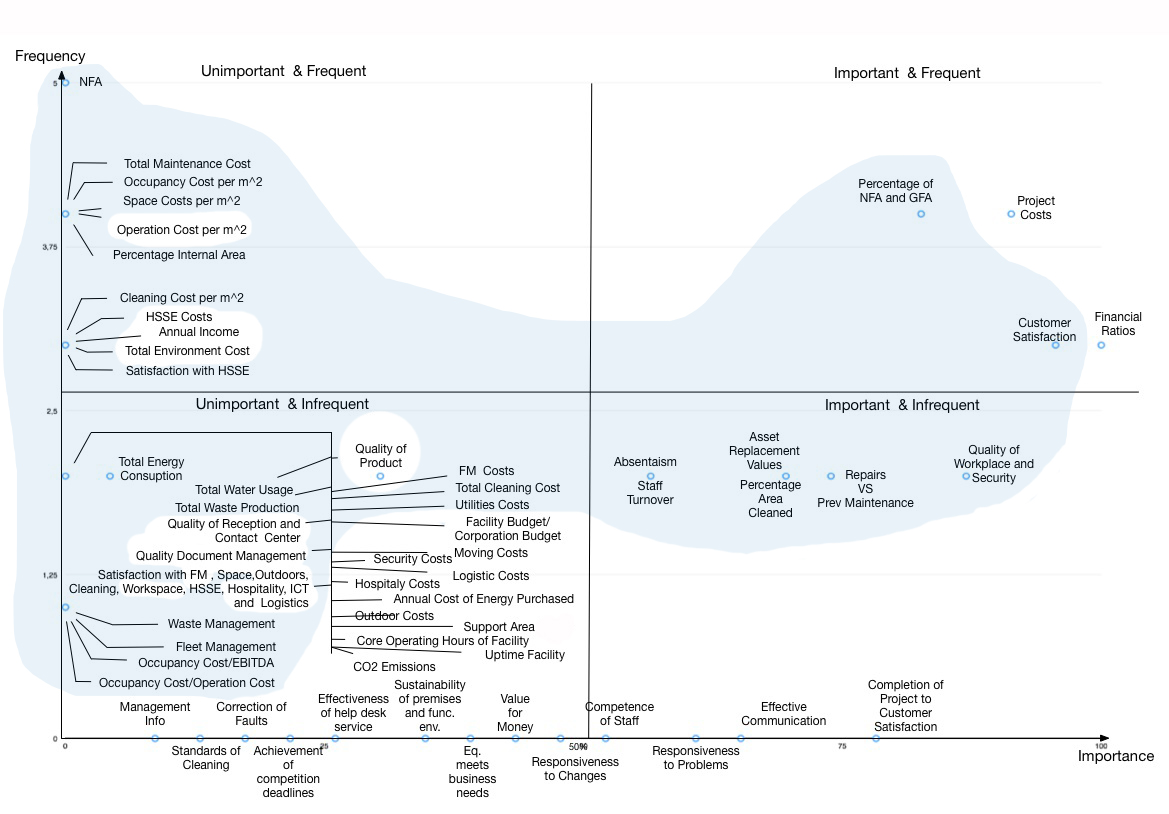
\includegraphics[width=1.1\textwidth]{img/importanceXfrequency10.jpg}
  %\end{adjustwidth}
  \caption{FM KPIs organized according to frequency and importance. Shaded area represents the options of an FM expert.}
  \label{fig:importanceXfrequency}
\end{figure}
In order to understand which were the most important KPIs for FM, it was needed to cross data between the various scientific literature and the existing solutions.
The Figure \ref{fig:importanceXfrequency} represents the information in tables \ref{tb:23KPIimportanceOrder}, \ref{tb:ListSpacialFinancialKPIpapers} and the KPIs given by the FM expert. In it, it is possible to visualize the most relevant KPIs based on importance and frequency. This graphic was constructed based on a cross-over of the KPIs described on the academic literature and the field experience of the FM expert. 



%Having regard the practical and theoretical level, the indicators on the shaded area of the figure are the best ones to compose the final list of indicators and will be used in the proposed solution.

 %So, of KPIs presented in Tables \ref{tb:ListSpacialFinancialKPIpapers} and \ref{tb:Resto2ListKPIpapers}, we could select only the most important ones. These KPIs are presented in Table \ref{tb:ListFinalKPI} and are the representatives of each dimension. 


%Some indicators have the same correspondent point on the graphic: {\bf [Note A] } Total Maintenance Cost, Occupancy Cost per $m^2$, Space Cost per $m^2$ and Operation Cost per $m^2$, {\bf [Note B]} Cleaning Cost per $m^2$, HSSE Costs, Annual Income, Total Environment Cost and Satisfaction with HSSE, {\bf [Note C]} Total Cleaning Cost, FM Costs, Utilities Costs, Facility Budget/Corporation Budget, Moving Costs, Security Costs, Logistic Costs, Hospitality Costs, Annual Cost of Energy Purchased, Outdoor Costs, Support Area, Core Operating Hours of Facility, Uptime Facility, CO2 Emissions, Total Water Usage, Total Waste Production, Quality of Cleaning, Quality of Reception and Contact Center, Quality of Document Management, Satisfaction with FM, Space, Outdoors, Cleaning, Workspace, HSSE,  Hospitality, ICT and Logistics, {\bf [Note D]} Occupancy Costs/Operation Costs, Occupancy Costs/EBITDA, Fleet Management and Waste Management. The indicators within the line are the ones chosen to be used on this document solution.

In order to be simpler to evaluate, a first iteration of the solution should use a short list of KPIs \cite{Costa2004}. The proposed list of KPIs for this project can be seen on Table \ref{tb:ListFinalKPI}.

\begin{table}[h!]%[t!]
	\vspace{0cm}
	\begin{adjustwidth}{-0.5cm}{0cm} 
	\resizebox{13cm}{!} {
	\begin{tabular}{llp{7cm}l}
		\hline
		 {\bf Indicator} &  {\bf Units/mo} & {\bf Description} \\
		\hline
		{\bf Financial Indicators} & & \\
		Total Cleaning Cost 				& \euro &  Sum of all cleaning costs \\
		Cleaning Cost per $m^2$ 			& \euro/$m^2$ &  Total Cleaning Cost/Net Room Area OR Total Cleaning Costs/Net Floor Area\\
		Total Maintenance Cost 				& \euro &  Sum of costs of maintenance for electricity equipment, HVAC, elevators, escalators, generators, UPS, ICT maintenance, etc\\  
		FM Costs 							& \euro &  Costs of FM department OR FM outsourcing \\
		Utility Costs 						& \euro  & Sum of costs for water, electricity, oil, gas and others \\
		Space Costs per $m^2$ 				& \euro/$m^2$ & Total Space Costs/Net Floor Area\\ 
		Occupancy Cost 						& \euro/$m^2$ & Total Occupancy Cost/Net Floor Area \\
		Occupancy Cost per Operation Costs & \% & (Occupancy Cost/Total Operation Costs)*100 \\
		Occupancy Cost per EBITDA & \% & (Occupancy Cost/Earning Before Interest, Taxes, Depreciation and Amortization)*100\\
		\hline

		{\bf Spacial Indicators} & & \\
		Net Floor Area per FTE				& $m^2$/FTE & Net Floor Area/Number of FTE personnel \\
		Percentage Net Floor Area 			& \% & (Net Floor Area/Total Level Area)x100 \\
		Percentage Internal Area			& \% & (Internal Area/Total Level Area)x100 \\
		Percentage Gross Floor Area 		& \% & (Gross Floor Area/Total Level Area)x100 \\
		\hline
		{\bf Maintenance/Cleaning Indicators} & &  \\
		Repairs VS Preventive Maintenance (by specialty)						& \% & (Number of Corrective Maintenance per month/Number of Preventive Maintenance per month)x100 \\
		Asset Replacement Values (by specialty)												& \% & (Annual Maintenance Cost/Maintained Assets Replacement Value)x100\\
		Percentage of Area Cleaned 												& \% & Area Cleaned/Net Floor Area \\
		\hline
		{\bf Productivity Indicators} & & \\
		Staff Turnover 	 			& \% & (Number of Employee Departures (FTE)/Average Number of Staff Members (FTE) Employed)x100\\
		Absenteeism  				& \% & (Total Days Lost/Total Possible Days Worked)x100 \\
		\hline

		{\bf Environmental Indicators} & & \\
		%CO2 emissions 						& tones/mo &  \\
		Total Energy Consumption	 		& kWh & \\
		Total Water Usage					& $m^3$ & \\
		Total Waste Production 				& tones & \\
		%Health and safety and environment 	&  & ? \\
		\hline
		 {\bf Service Quality Indicators} &  &  \\ 
		Quality of Cleaning							&  & Values Obtained Through Audits or Questionnaires \\
		Quality of Workplace 						&  & Values Obtained Through Audits or Questionnaires \\
		Quality of Security 						&  & Values Obtained Through Audits or Questionnaires \\
		\hline
		{\bf Satisfaction Indicators} & & \\
		Client Satisfaction 			& \% & Values Obtained Through Questionnaires \\
		Satisfaction with Space			& \% & Values Obtained Through Questionnaires \\
		Satisfaction with Cleaning 		& \% & Values Obtained Through Questionnaires \\
		Satisfaction with HSSE			& \% & Values Obtained Through Questionnaires \\
		\hline
	\end{tabular}
	}
	\end{adjustwidth}
\caption{List of Final Normalized KPIs that will be used on final solution, after validation by several FM experts.}
\label{tb:ListFinalKPI}
\end{table}
			
%!TEX root = ../report.tex

% 
% Architecture
% 

\section{Solution Proposal} 
\label{solutionproposal}

As referred before, it is necessary a new solution where different organizations, with different FM systems, would be able to visualize their FM results through a graphical illustration of their KPIs. The most important fact here will be the aggregation of information of different organizations, that will be compared between them, bringing a better insights where your organization is in terms of FM relatively to others. Organizations will then be ranked by their results, but their information will never be shown to others, being the results always classified.

\subsection{Overview}

The solution will be developed as a Web Application, which will be divided in two parts. Server side and Client side. The server side will run directly on the hosting servers, while the client side will run on the browser as an endpoint to the server.
The solution will:


\begin{itemize}
	\item Use authentication service to authenticate the users of a organization
	\item Display KPIs through graphics		
	\item Have a ranking between organizations
	\item Have a cache on the database for better performance
\end{itemize}

This document solution architecture overview can be found on Figure \ref{fig:architecture}. 

\begin{figure}[t!]
  \centering
  %\begin{adjustwidth}{-3cm}{0cm}
  %\begin{sideways}
  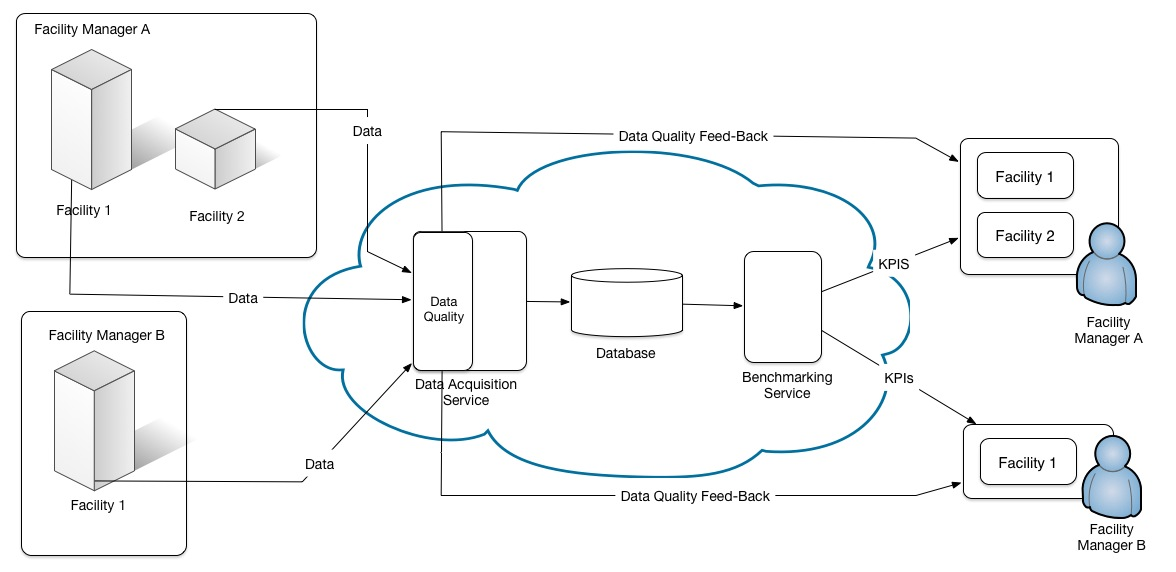
\includegraphics[width=1\textwidth]{img/OrganizacaoGeral.jpg}
  %\end{sideways}
  %\end{adjustwidth}
  \caption{FM benchmarking system architecture. Organizations send their data on a standard format, to be stored on a database. This info is then accessed by different users representatives of each organization.}
  \label{fig:architecture}
\end{figure}

\subsection{Architecture}

\begin{description}
	\item  [Client Side] The Client Side application will be running on the browser of the user connecting to the website. This application will have to display an interface so that the user can interact with the application and where the statistics about the organization will be presented. It will be used  Bootstrap Framework for the web site design which enables a quicker development and permits an adaptive front-end for mobile devices. For the generation of the graphics will be used the javascript library highcharts and if necessary the D3.js for more complex graphics.\\

	\item [Server Side] The Server Side will be running the application and will be the responsible for the processing and storage of the data sent by the Organization to the DB. It will also be responsible for organizations and users management, authentication and data management and update (CRUD - Create, Read, Update and Delete). For the Server Side will be used the Play Framework which is also responsible for the generation of HTML templates that will be sent to the Client Side.\\

	\item [Database] It will be used a relational Database (DB), that will be theoretically divided in three: Input Data Staging Area, KPI Aggregated Data and Facility Metadata as can be seen in Figure \ref{fig:db}. The Input Data Staging Area stores the data sent by the organization. The KPI Aggregated Data uses the Input Data Staging Area data to calculate the KPIs and store them.
	Without this division there would be necessary heavier queries and consequently the system would be slower. In order to deliver KPI information in real-time, the KPI Aggregated Data caches the computed information gathered by the Input Data Staging Area, making the system quicker.

	%If the KPIs would be calculated only when a client queries that specific information, it would have been a problem: when many clients asks for more heavy data queries, the system will be overloaded. Using this system of previous calculation of the KPIs, this heavy queries will be replaced for more simple queries and the calculation of each KPI will occur only once. This will not overload the system and the performance will be better.
\end{description}

\begin{figure}[t!]
  \centering
  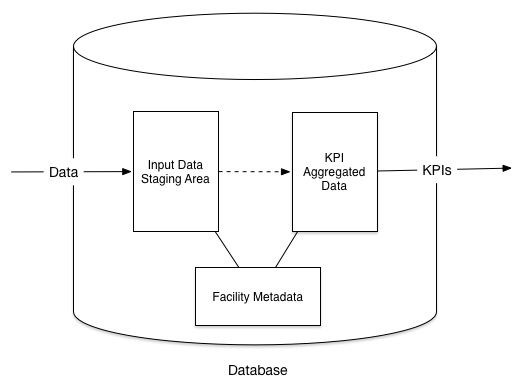
\includegraphics[width=0.70\textwidth]{img/DataBase.jpg}
  \caption{Database arrangement overview. It receives the data and stores it on Input Data Staging Area, then, when the KPIs are calculated they are stored at KPI Aggregated Data.}
  \label{fig:db}
\end{figure}

%--------------------------------------------Acabou--------------------------------
%----------------------------------------------------------------------------------
\iffalse
\begin{figure}[t!]
  \centering
  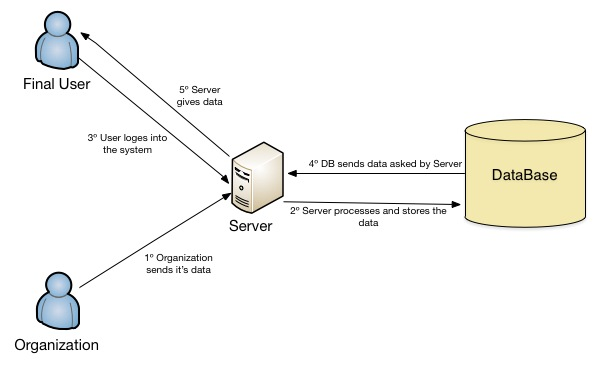
\includegraphics[width=0.95\textwidth]{img/Arquitectura.jpg}
  \caption{System Specific Architecture. }
  \label{fig:architecture}
\end{figure}

\paragraph{\bf Organization Server} \hspace{0pt} \\ The Organization Server will be a server installed on the organization. On this server each organization can subscribe the users that they want. This server will have an authenticated communication with the Central Server, and will be through it that the data will be transfered to the Central Server.

---
Organizations sends their data to the Server that is responsible for the process and store of it to the DB. Users can ask for the information stored, but for that, they have to be authenticated on the Web Application. Then, the Server asks and sends the data to the specific client.
----

\subsection{Implementation}

\begin{itemize}
	\item DB dividida dados/index
	\item que db usar?
	\item na cloud
	\item interface a utilizar
	\item que tipo de interface - o que usar?
	\item recebe dados, calcula logo os index e guarda-os
	\item Como calcular os index - kpis importantes
	\item que dados recebe e que index são calculados
\end{itemize}
\fi
%!TEX root = ../report.tex

% 
% Evaluation
% 

\section{Evaluation}
\label{Evaluation}

This works validation involves the development of a proof of concept (POC) to prove its usability and claims. This concept will storage organizations data, calculate correspondent KPIs and display it through several graphics. It also creates a raking between the different organizations FM results. 
In order to validate the proposed solution, will be performed a set of tests:

\begin{description}
	\item [Usability Tests] evaluates the application by testing it with users. It provides a direct perception how the users interact with the application, the common errors they make and if they can execute the tasks. As a result of this test, we can understand if the application interface is well designed and perceptible.\\

	\item [Qualitative Tests] combined with the usability tests, are possible to gather users opinions. They can help find better ways to improve the application interface.\\

	\item [Indicators Rating] is very important to realize which indicators are the most convenient to any specific users. This can be achieved by a questionnaire or by integrating an indicator rating tool inside the application, where the users can select their preferable indicators.\\

	\item [Performance Tests] in order to test the cache efficiency on the database. Will be made two tests. For the first test, KPIs will be asked directly to the Input Data Staging Area, on the second test, it will be used a cache, and the KPIs will be asked to the KPI Aggregated Data. This way, it is possible to understand the performance optimization brought by the cache. 
\end{description}

%It will be used a web frameworks and a public or private cloud provider.

%Finally, this work evaluation concludes by inquiring industry organizations through an online survey, to validate this work claims and solution proposal. It’s expected that this validation can prove the claims and conclusions of this work and enhance it credibility.

\subsection{Deployment}
To provide a real situation evaluation and benchmarking, this POC will be deployed on the cloud provider Heroku. Heroku is a PaaS which provides SQL Postgres Database and a Github integration, which permits a quicker and easier deployment of the application while allowing vertical and horizontal scalability on the fly \cite{Heroku}. 


\section{Planning}
\label{Planning}

This document project will follow the methodology depicted on the Gantt Chart of the Figure \ref{fig:PlaneamentoTese}, which can be seen an overall view of the time line of this thesis work.

\begin{figure}[h!]
  \centering
  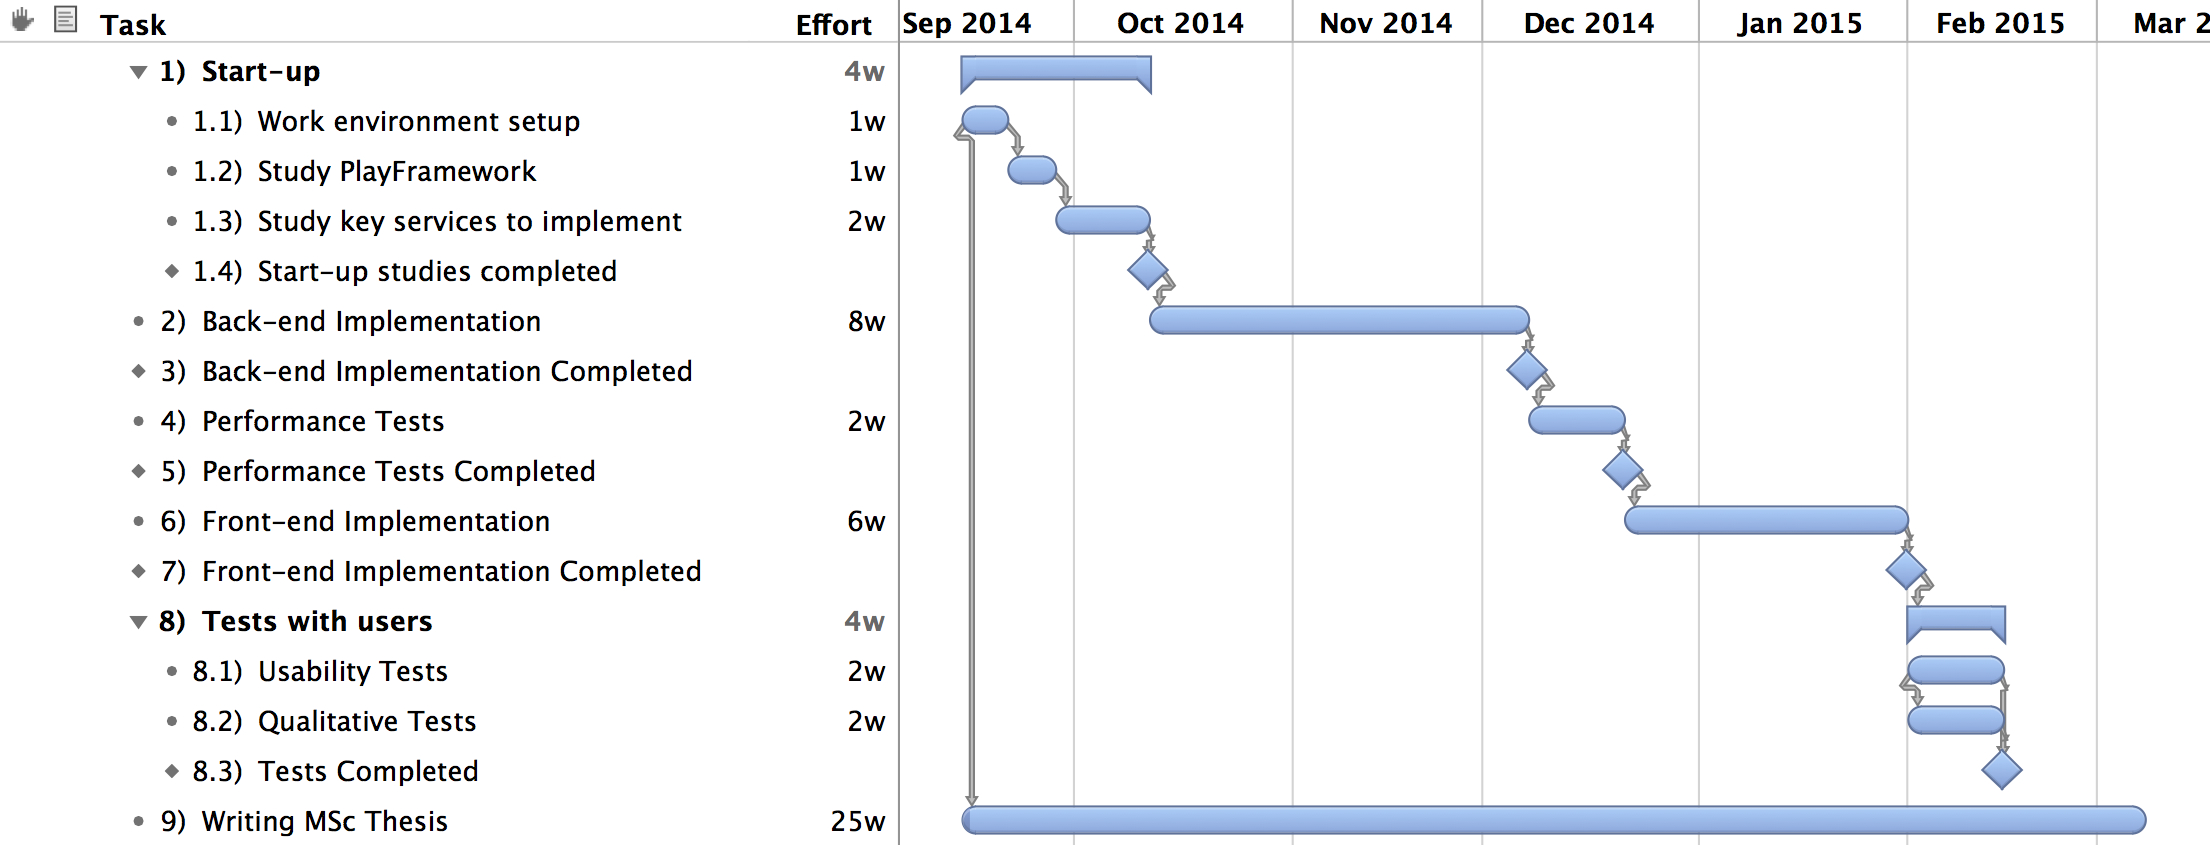
\includegraphics[width=1\textwidth]{img/PlaneamentoTese.jpg}
  \caption{Project Gantt Chart. Task planning and working time estimation.}
  \label{fig:PlaneamentoTese}
\end{figure}



%!TEX root = ../report.tex

% 
% Conclusions
% 

\section{Conclusions}
Nowadays the lack of accurate metrics which drives decision-making, makes the achievement of an effective portfolio and operations management a challenge.
This report proposes a new FM benchmarking cloud application for presenting KPIs and a ranking FM organizations. First, was introduced the concepts of FM benchmarking, the problem to be solved by this document solution and the motivation for it. Then, is described with more detail the concepts of FM, Benchmarking, KPIs and Cloud-Computing. Afterwards, is described the different Standards used nationally and internationally, the related work done by other researchers in the field of FM benchmarking, and some technologies existent today in this area. Then, is specified the architecture of the cloud application proposed. Finally it is described how the solution will be evaluated. 

With the solution proposed in this project, quantifying real property performance will be easier and organizations will have a better way to evaluate its own FM metrics, while enabling the comparison of metrics between enterprises and facilities.

%We have to have in account developing a benchmarking strategy selecting only organizations within their own industry to benchmark against \cite{Roka-Madarasz2010}, because comparisons across different categories may estimate the potential that exist for improvement.


\bibliographystyle{ieeetr}
\bibliography{books,library} 
\newpage
\appendix
%!TEX root = ../report.tex

\section{Appendix} % (fold)
%\label{sec:attachments}
\setcounter{table}{0} \renewcommand{\thefigure}{A.\arabic{figure}}

\begin{table}[h!]
	\vspace{0cm}
	\begin{adjustwidth}{3cm}{0cm}
	\resizebox{6cm}{!} {
	\begin{tabular}{l}

		\hline
		{\bf {\emph{Indicator}}} \\
		\hline
		{\bf {\emph{Description of Facilities}}} \\
		Industries represented \\
		Facility use \\
		%Ownership \\ 
		Hours of operation \\ 
		Number of occupants \\ 
		%Location of facility \\ 
		\hline

		{\bf {\emph{Sizes and Uses of Facilities}}} \\
		Gross area \\
		Rentable area \\ 
		Usable area \\ 
		Square footage per occupant \\ 
		Building efficiency rates \\ 
		Workstation utilization rates \\ 
		Office space per worker \\ 
		Support area \\ 
		\hline

		{\bf {\emph{Office Space Planning}}} \\
		Vacancy rates \\
		Space allocation policies \\ 
		Office type and size \\ 
		\hline

		{\bf {\emph{Relocation and Churn}}} \\
		Organizational moves \\
		Cost of moves \\ 
		Churn rate \\ 
		\hline

		{\bf {\emph{Maintenance, Janitorial and Indirect Costs}}} \\
		Organizational moves \\
		 Maintenance costs (by age of facility) \\ 
		 Percentage of replacement cost \\
		Repair vs preventive maintenance \\ 
		 Outsourcing of maintenance function \\
		 Janitorial costs \\ 
		 Indirect costs \\ 
		\hline

		{\bf {\emph{Utility Costs}}}\\
		Utility costs \\
		Utility usage \\ 
		\hline

		{\bf {\emph{Environmental and Life Safety Costs}}}\\
		Environmental costs \\
		Life-safety costs \\ 
		\hline

		{\bf {\emph{Support and Project Costs}}}\\
		Security costs \\
		Project costs \\
		Space planning costs \\ 
		Employee amenities costs \\ 
		\hline

		{\bf {\emph{Financial Indicators}}}\\
		Replacement value of facility \\
		Lease type and cost \\
		Cost of operations \\ 
		Cost of providing the fixed asset \\ 
		Occupancy cost \\ 
		Financial ratios \\ 
		Total annual financial costs \\ 
		\hline
	\end{tabular}
	}
	\end{adjustwidth}
\caption{Key Performance Indicators for FM organized by areas within facilities operation according to IFMA \cite{Roka-Madarasz2010}.}
\label{tb:TableKPIFMBenchmarking}
\end{table}

\begin{table}[h!]
	\begin{adjustwidth}{3cm}{0cm}
	\begin{tabular}{l}
		\hline
		{\bf {\emph{Activities and Reports}}} \\
		\hline
		{\bf {\emph{Space Management}}}\\
		Rooms by building \\
		Synchronize room percentages \\
		Highlight rooms by department \\ 
		Financial statement for charge-back \\ 
		Actual cost vs. budgets for departments \\ 
		Historical space usage by department \\ 
		\hline

		{\bf {\emph{Asset Management}}}\\
		Equipment standards and inventory  \\
		Depreciation schedules for assets \\
		Equipment disposition history \\ 
		\hline

		{\bf {\emph{Operations and Maintenance}}}\\
		Work orders scheduled vs. completed \\
		Rooms with active work orders \\
		Service level agreements \\ 
		Parts usage history \\ 
		Planning board for labor resources \\ 
		\hline

		{\bf {\emph{Capital Budgeting}}}\\
		Approved projects by funding year\\
		Available capital and expense funds \\
		Budget by program \\ 
		\hline

		{\bf {\emph{Geo-spatial Views}}}\\
		Facilities and site infrastructure master planning \\
		Utilities, cable plant and network management \\
		Environmental health and safety compliance \\ 
		Emergency preparedness and response \\ 
		\hline


	\end{tabular}
	\end{adjustwidth}
\caption{List of reports of the ARCHIBUS FM \cite{ARCHI} software package for Educational Institutions organized by category.}
\label{tb:ARCHIBUSListActReports}
\end{table}


\begin{table}[t!]
	\vspace{0cm}
	\begin{adjustwidth}{0cm}{0cm} 
	\begin{tabularx}{\textwidth}{l|X|X|X|X|X}
		\hline
		{\bf Routine Cleaning} &  {\bf 0\%} & {\bf 25\%} & {\bf 50\%} & {\bf 75\%} & {\bf 100\%} \\
		\hline
		\multicolumn{1}{  l|  }{\multirow{2}{*}{Workspace Frequency}} &	1x per week &	2x per week &	3x per week & 4x per week &	every day\\
		\cline{2-6}
		& & & & &\\
		\hline
		\multicolumn{1}{  l|  }{\multirow{2}{*}{Toilets Frequency}} &	$<$ 2x per week &	2-3x per week &	every day	& 2x per day	& $>$ 2x per day \\
		\cline{2-6}
		& & & & &\\
		\hline
		\multicolumn{1}{  l|  }{\multirow{2}{*}{Staff Supervision}} &	poor supervision by area managers & & acceptable supervision by area managers & & expert supervision by area managers \\
		\cline{2-6}
		& & & & &\\
		\hline
		\multicolumn{1}{  l|  }{\multirow{2}{*}{Cleaning Standard}} & very inconsistent and of poor standard (noticeably unclean on inspection) &	usually inconsistent and below standard (numerous issues to action on inspection) &	consistently to an acceptable standard (issues to action on inspection) & usually consistent of a high standard (few issues to action on inspection) &	always consistent and of high standard (very clean on inspection) \\
		\cline{2-6}
		& & & & &\\
		\hline
		\multicolumn{1}{  l|  }{\multirow{2}{*}{Customer Service}} & cleaning staff are impolite and not very helpful & cleaning staff are polite, but not very helpful & cleaning staff are polite and helpful &	cleaning staff are proactive in offering service & cleaning staff go above and beyond the call of duty \\
		\cline{2-6}
		& & & & &\\
		\hline
		\multicolumn{1}{  l|  }{\multirow{2}{*}{Staff Presentation}} & cleaning staff look untidy and are often out of uniform & & cleaning staff look acceptable and occasional exceptions are promptly rectified & & cleaning staff look tidy and are always in uniform \\
		\cline{2-6}
		& & & & &\\
		\hline
		\multicolumn{1}{  l|  }{\multirow{2}{*}{User Complaints}} & monthly complaints/staff base $>$20\% & monthly complaints/staff base = 15-20\% &	monthly complaints /staff base = 10-15\% &	monthly complaints/staff base = 5-10\% & monthly complaints/staff base <5\%\\
		\cline{2-6}
		& & & & &\\

		\hline
	\end{tabularx}
	\end{adjustwidth}
\caption{Example of Routine Cleaning Quality Questionnaire. The percentages correspond to: 0\% - very poor, 25\% - poor, 50\% - average, 75\% - good, 100\% - very good. Personnel should select the option closest to their situation.}
\label{tb:RoutineCleaningQuesitonnarie}
\end{table}

\begin{table}[t!]
	\vspace{0cm}
	\begin{adjustwidth}{0cm}{0cm} 
	\begin{tabularx}{\textwidth}{l|X|X|X|X|X}
		\hline
		{\bf Special Cleaning} &  {\bf 0\%} & {\bf 25\%} & {\bf 50\%} & {\bf 75\%} & {\bf 100\%} \\
		\hline
		\multicolumn{1}{  l|  }{\multirow{2}{*}{Flooring Frequency (deep cleaning)}} & $<$ 2x per annum &	2x per annum & 3x per annum & 4x per annum & $>$ 4x per annum\\
		\cline{2-6}
		& & & & &\\
		\hline
		\multicolumn{1}{  l|  }{\multirow{2}{*}{Partitions Frequency}} & $<$2x per annum & 2x per annum &	3x per annum & 4x per annum	& $>$4x per annum\\
		\cline{2-6}
		& & & & &\\
		\hline
		\multicolumn{1}{  l|  }{\multirow{2}{*}{Windows Frequency}} &	$<$2x per annum & 2x per annum & 3x per annum &	4x per annum & $>$ 4x per annum\\
		\cline{2-6}
		& & & & &\\
		\hline
	\end{tabularx}
	\end{adjustwidth}
\caption{Example of Special Cleaning Quality Questionnaire. The percentages correspond to: 0\% - very poor, 25\% - poor, 50\% - average, 75\% - good, 100\% - very good. Personnel should select the option closest to their situation.}
\label{tb:SpecialCleaningQuesitonnarie}
\end{table}



% 
% Bibliography
% 

%\bibliographystyle{plain} 

\end{document}